%%%%%%%%%%%%%%%%%%%%%%%%%%%%%%%%%%%%%%%%%%%%%%%%%%%%%%%%%%%%%%%%%%%%%%%%%%%%%%%
\chapter{Pesquisa em memória secundária}
%%%%%%%%%%%%%%%%%%%%%%%%%%%%%%%%%%%%%%%%%%%%%%%%%%%%%%%%%%%%%%%%%%%%%%%%%%%%%%%

Este capítulo aborda questões relacionadas a técnicas de armazenamento
e recuperação de dados em memória secundária.

%%%%%%%%%%%%%%%%%%%%%%%%%%%%%%%%%%%%%%%%%%%%%%%%%%%%%%%%%%%%%%%%%%%%%%%%%%%%%%%
\section{Memória secundária}
%%%%%%%%%%%%%%%%%%%%%%%%%%%%%%%%%%%%%%%%%%%%%%%%%%%%%%%%%%%%%%%%%%%%%%%%%%%%%%%

A classificação de dispositívos físicos pode ser feita ao considerar:
\begin{enumerate}
\item Desempenho no acesso aos dados.
\item Custo por unidade de dados.
\item Confiabilidade para casos de perda de dados em falhas de
energia ou falha do sistema, ou mesmo falha física do dispositívo.
\end{enumerate}
Também pode-se diferenciar armazenamento em:
\begin{description}
\item[Volátil] perde dados quando é desligado.
\item[Não-volátil] persistente mesmo quando é desligado. Inclui armazenamento
secundário e terciário.
\end{description}

%%%%%%%%%%%%%%%%%%%%%%%%%%%%%%%%%%%%%%%%%%%%%%%%%%%%%%%%%%%%%%%%%%%%%%%%%%%%%%%
\subsection{Mídias de armazenamento}

As médias de armazenamento disponíveis em geral são:
\begin{description}
\item[Cache] a mais rápida e custosa, volátil, e gerenciada pelo hardware
do processador.

\item[Memória principal] acesso rápido da ordem de 10 a 100 nanosegundos (1 nanosegundo = $10^{-9}$).
Em geral muito pequena (ou muito cara) para armazenar todos os dados de um banco de dados.
Hoje  em dia, em alguns casos, armazena todo o banco de dados (\emph{memcached}).
Ela é volátil, sendo que os dados são perdidos na falta de energia ou falha do sistema.

\item[Flash] dados sobrevivem em falhas de energia. Dados podem ser escritos em um local
uma única vez, porém podem ser escritos novamente.
Pode ser lida um número ilimitado de vezes, mas há um limite no  número de gravações
que varia entre 10K e 1M.
As leituras podem ser mais rápidas que a memória principal, mas as escritas
são lentas.
Muito usada em dispositivos embarcados como câmeras digitais, 
telefones, e memórias flash drive (pendrive).

\item[Magnética] dados são armazenados em uma mídia magnética com discos de movimento
giratório. 
Deve-se ler os dados do disco para a memória principal, e depois escrever de volta ao disco.
O acesso direto é possível em qualquer ordem, ao contrário de mídias de fita.


\item[Ótica] não volátil e os dados são lidos óticamente de um disco 
giratório através de um laser.
Os mais populares são CD-ROM (640 MB), DVD (4.7GB), e Blu-ray (27 GB a 54 GB).
As leituras e escritas são mais lentas comparadas a discos magnéticos.

\item[Fita magnética]
não volátil, usado primariamente para backup (recuperar falhas de disco), e 
arquivamento de dados.
O acesso é sequencial, muito mais lento que discos. Porém, a capacidade
de armazenamento é alta (40 a 300GB).
\end{description}

A figura~\ref{aula06:fig:media} ilustra a hierarquia de armazenamento de acordo com 
o desempenho e custo.
Os níveis mais altos são mais custosos, porém mais rápidos.
No sentido contrário, o custo por bit reduz, mas o tempo de acesso aumenta.
%
\begin{figure}[!htb]
\centering
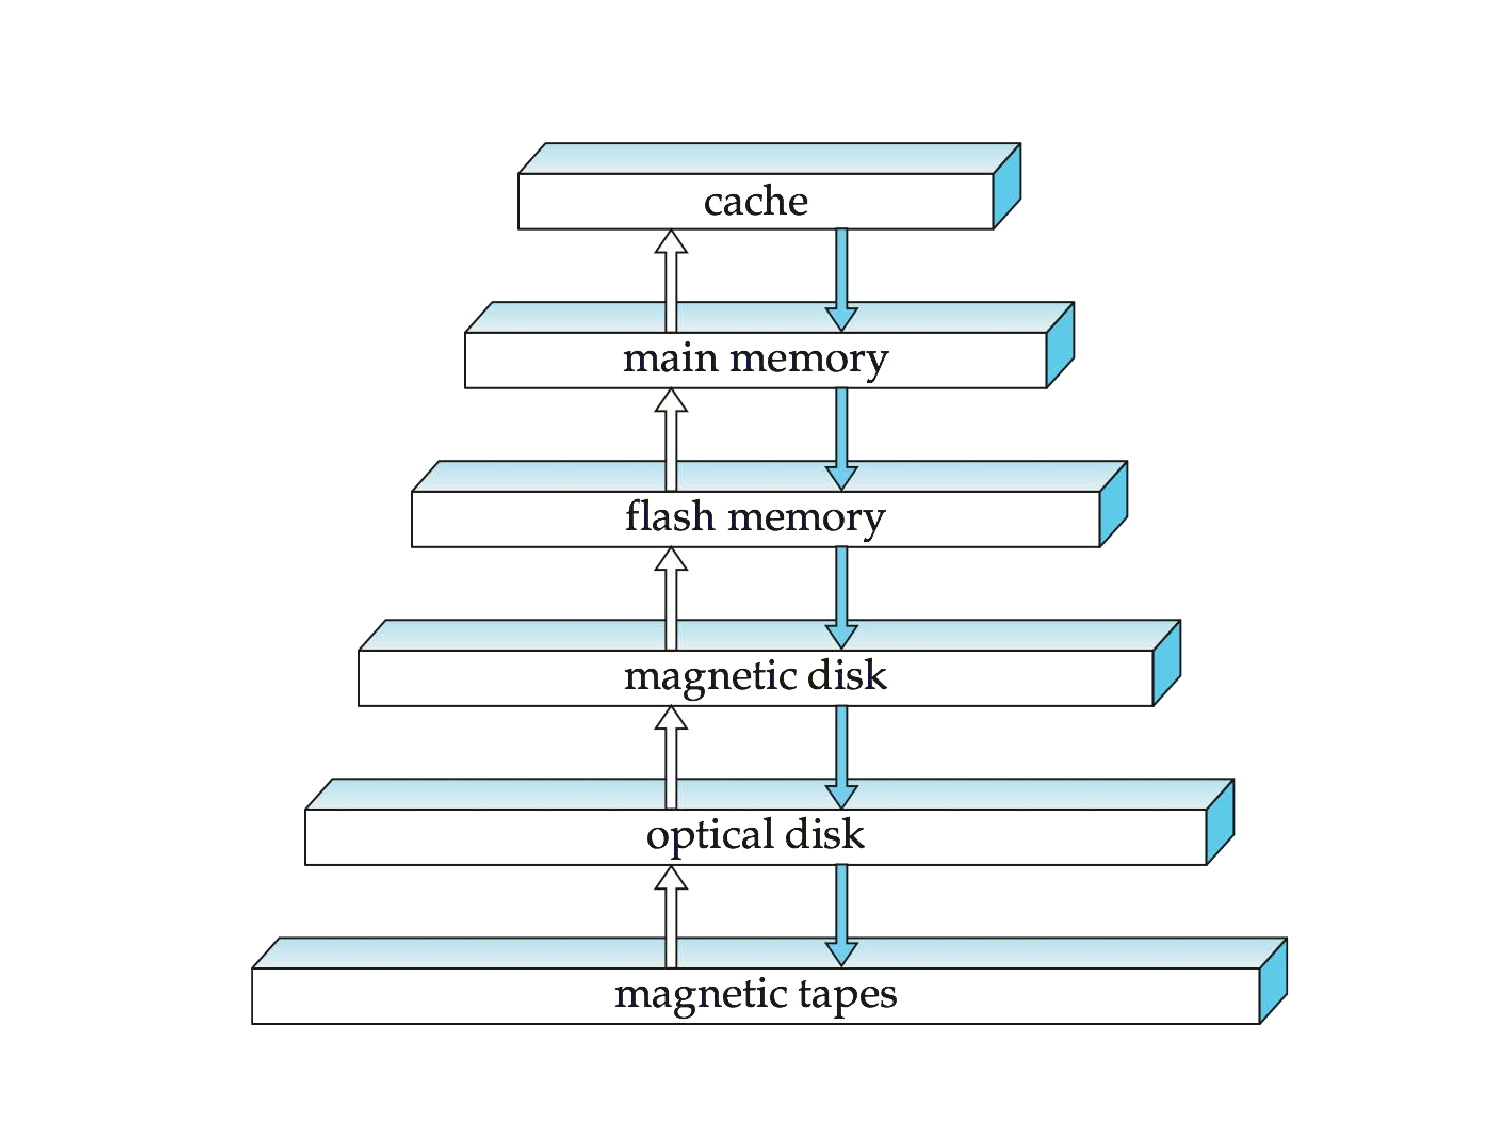
\includegraphics[width=0.6\textwidth]{aula06-media}
\caption{Hierarquia de mídias de armazenamento.}
\label{aula06:fig:media}
\end{figure}

Nessa hierarquia, podemos agrupar as mídias em:
\begin{description}
\item[Armazenamento primário] mais rápido mas volátil. Ex: cache, memória principal.

\item[Armazenamento segundário] próximo nível na hierarquia, não volátil,
acesso moderadamente rápido. Ex: memória flash, discos magnéticos.

\item[Armazenamento terciário] nível mais baixo, não volátil, tempo de acesso
lento. Também chamado armazenamento \emph{off-line}. Ex: fita magnética, armazenamento ótico.
\end{description}

%%%%%%%%%%%%%%%%%%%%%%%%%%%%%%%%%%%%%%%%%%%%%%%%%%%%%%%%%%%%%%%%%%%%%%%%%%%%%%%
\subsection{Disco magnético}

\subsubsection{Estrutura física}

Fisicamente, discos magnéticos são simples.
A figura~\ref{aula06:fig:hd} mostra o funcionamento interno de um disco.
%
\begin{figure}[!htb]
\centering
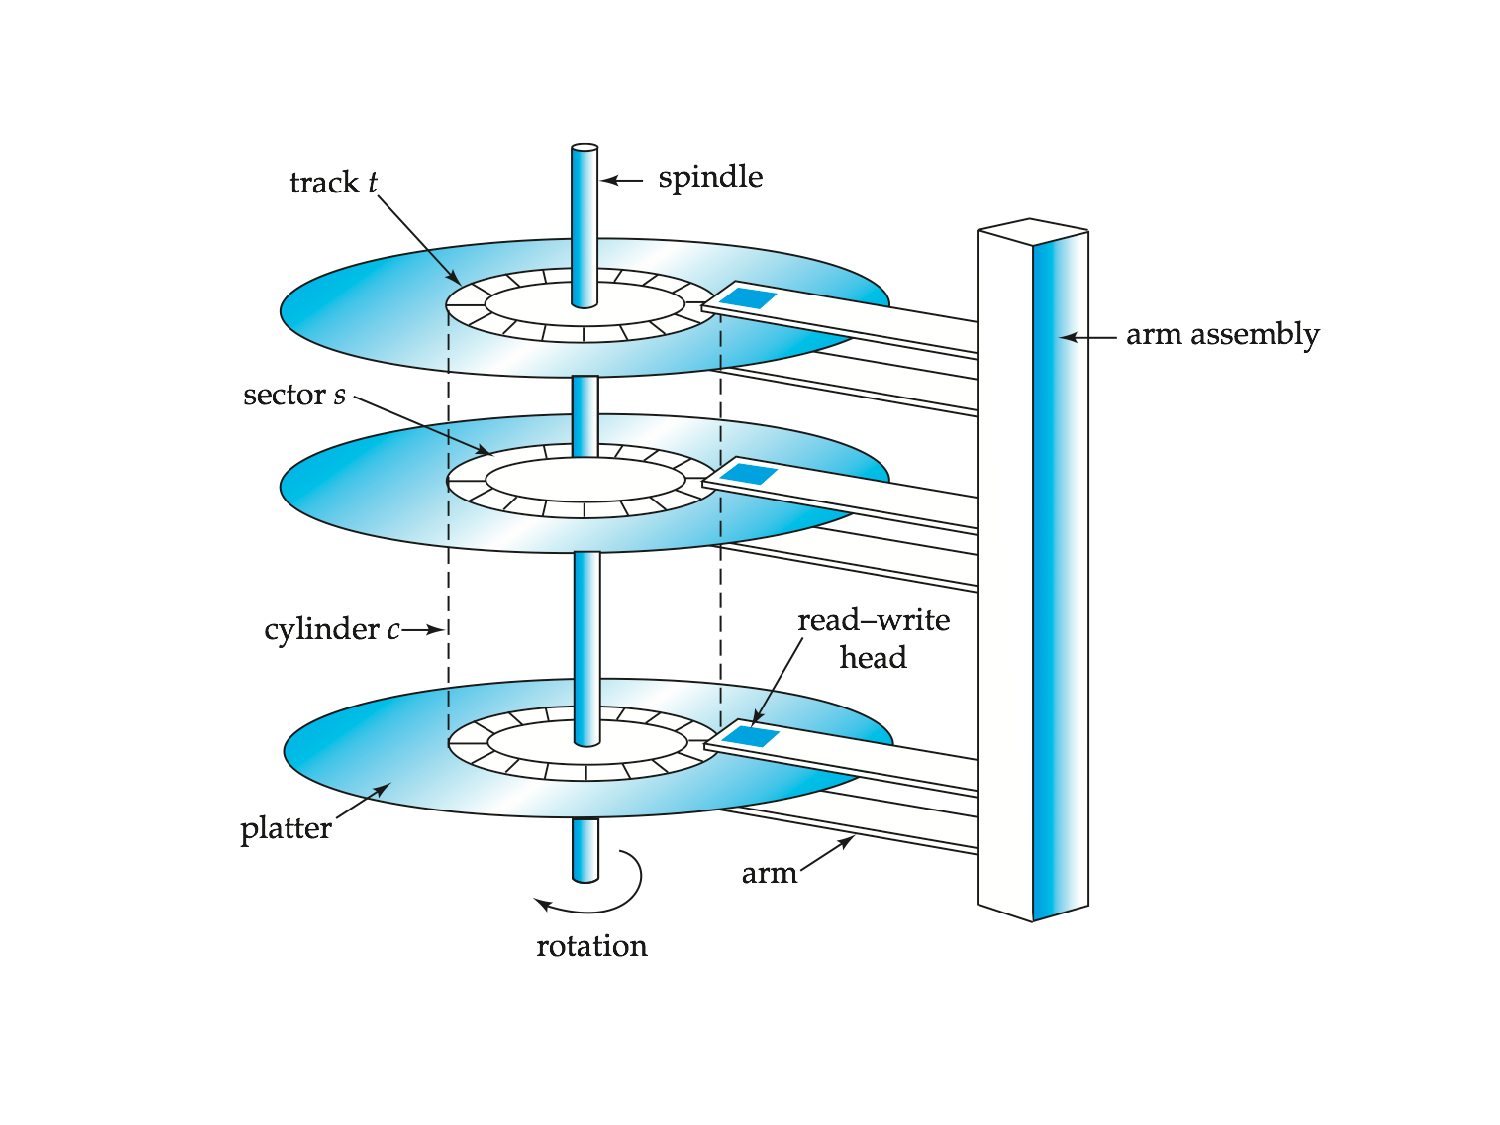
\includegraphics[width=0.6\textwidth]{aula06-hd}
\caption{Mecanismo de cabeças de leitura em um disco magnético.}
\label{aula06:fig:hd}
\end{figure}

Cada prato do disco tem duas superfícias com material magnético, onde a informação
é gravada.
O cabeçote de escrita-leitura (\emph{read-write head}) fica posicionada bem 
próxima a superfície do prato, e lê e escreve dados codificados magneticamente.
A superfície é dividida logicamente em {\bf trilhas}, que são subdivididas em 
\textbf{setores}. 
Um setor é a menor unidade que pode ser lida ou escrita do disco.
Em geral, um setor tem 512 bytes; há perto de 50K a 100K trilhas por prato, e 1
a 5 pratos por disco.

Os pratos são montados em braços de disco.
Para ler e escrever um setor, o braço do disco se move para posicionar o cabeçote
na trilha correta.
O prato gira, e os dados são lidos e/ou escritos a medida que o setor
passa pelo cabeçote.

Outro componente de discos é o {\bf controlador de disco} que faz a inteface 
entre o computador e o hardware do disco.
Ele aceita comandos de alto nível para ler e escrever setores.
Entre outras funções, garante checagem de erros.

\subsubsection{Medidas desempenho}

O \textbf{tempo de acesso} é o tempo que leva desde a solicitação de leitura/escrita
até o momento em que a transferência começa de fato. 
O tempo de acesso consiste em:
\begin{description}
\item[Tempo de busca] tempo que leva para reposicionar o braço na trilha correta.
O tempo médio de busca é 1/2 do pior tempo de busca, em geral 4 a 10 milisegundos.

\item[Latência rotacional] tempo que leva para o setor a ser acessado
aparecer debaixo do cabeçote. Latência média é 1/2 do pior caso, em geral
4 a 11 milisegundos em discos (5400 a 15000 rpm). 
\end{description}

A \textbf{taxa de transferência} é a taxa com que os dados são recuperados ou 
armazenados no disco. A taxa máxima é de 25 a 100 MB por segundo, e essa
taxa é menor para trilhas internas.

O \emph{Mean time to failure} (MTTF) é o tempo médio de funcionamento de um disco
sem falhas. 
Esse tempo varia entre 3 a 5 anos. 
A probabilidade de falhas em disco novos é baixa, que corresponde a um
``MTTF teórico'' de 500K a 1,2M horas.
Ou seja, um MTTF de 1,2M horas para um disco novo significa que dados 1000 novos discos,
na média um irá falhar a cada 1200 horas.

\subsubsection{Otimização de acessos}

A transferência de dados entre disco e memória ocorre em unidades de \textbf{blocos},
que são uma sequência continua de setores em uma única trilha.
O tamanho varia de 512 a vários kilobytes. Blocos pequenos podem implicar 
em várias transferencias do disco, enquanto que grandes blocos podem 
desperdiçar espaços devido a blocos parcialmente ocupados.
Um tamanho típico utilizado é de 4 a 16 kilobytes.

A otimização de acessos envolve \textbf{algoritmos de escalonamento} que são usados para ordenar o 
acesso às trilhas para minimizar o  movimento do braço.
O \textbf{algoritmo do elevador} funciona da seguinte forma:
\begin{enumerate}
\item move o braço do disco em uma direção (de dentro para fora ou de fora para dentro).
\item processa todas as requisições pendentes nessa direção.
\item reverte o movimento e repete a varredura.
\end{enumerate}

Outra forma de otimização é a \textbf{organização de arquivos} que otimiza o acesso ao
organizar os blocos, de modo a corresponder à forma com que os dados são acessados.
Exemplo é armazenar informações relacionadas em regiões próximas.
Arquivos podem se \textbf{fragmentar} com o passar do tempo.
Fragmentação acontece quando o arquivo é modificado, ou quando os blocos livres
estão espalhados, e novos arquivos tiverem que ocupar esses blocos.
O acesso sequencial a um arquivo fragmentado leva a maior movimentação do
braço do disco. 
Alguns sistemas possuem utilitários para \textbf{desfragmentar} o sistema
de arquivos, de modo a acelerar o acesso.

%%%%%%%%%%%%%%%%%%%%%%%%%%%%%%%%%%%%%%%%%%%%%%%%%%%%%%%%%%%%%%%%%%%%%%%%%%%%%%%
\section{Organização de arquivos}
%%%%%%%%%%%%%%%%%%%%%%%%%%%%%%%%%%%%%%%%%%%%%%%%%%%%%%%%%%%%%%%%%%%%%%%%%%%%%%%

A pesquisa em memória secundária normalmente está associada a \textbf{pesquisa 
em bancos de dados}.
O banco de dados é armazenado como uma coleção de arquivos. Cada arquivo
é uma sequência de registros, e cada registro é uma sequência de campos.

%%%%%%%%%%%%%%%%%%%%%%%%%%%%%%%%%%%%%%%%%%%%%%%%%%%%%%%%%%%%%%%%%%%%%%%%%%%%%%%
\subsection{Registros de tamanho fixo}

A estratégia mais simples é assumir \textbf{registros de tamanho fixo}.
Cada tabela possui o seu próprio arquivo, e cada arquivo possui registros
de um tipo específico de dado.
O cabeçalho possui informações de controle. Cada registro tem um ponteiro
especial, que aponta para o seu próximo registro.
O problema com essa abordagem é a ocupação parcial do bloco.
Por exemplo, cada registro ocupa 300 bytes e cada bloco ocupa 1024 bytes.
O cabeçalho ocupa 20 bytes. Qual o mínimo de espaço que será desperdiçado ?

Uma solução é permitir que registros cruzem a fronteira de um bloco. 
As alternativas para remoção do registro $i$ são:
\begin{enumerate}
\item mover registros $i+1$, ..., $n$ para $i$, ..., $n-1$.
\item mover registro $n$ para $i$.
\item não mover nada, ligar os registros vazios por uma \emph{free list}.
\end{enumerate}

Com \emph{free lists}, pode-se usar um ponteiro especial para guardar os registros livres.
Ela é uma representação mais eficiente que reusa o espaço destinado
aos atributos dos registros para guardar os ponteiros.
O cabeçalho possui informações de controle como ponteiro para o primeiro registro
com dados do bloco, e ponteiro para o primeiro registro livre do bloco.

O principal problema dessa abordagem é o desperdício de espaço dentro do bloco.

%%%%%%%%%%%%%%%%%%%%%%%%%%%%%%%%%%%%%%%%%%%%%%%%%%%%%%%%%%%%%%%%%%%%%%%%%%%%%%%
\subsection{Registros de tamanho variável}

A estrutura de \textbf{slotted-page} é comumente utilizada para organizar
registros de tamanho variável dentro de um bloco.
A figura~\ref{aula06:fig:slotted} ilustra a estrutura.
%
\begin{figure}[!htb]
\centering
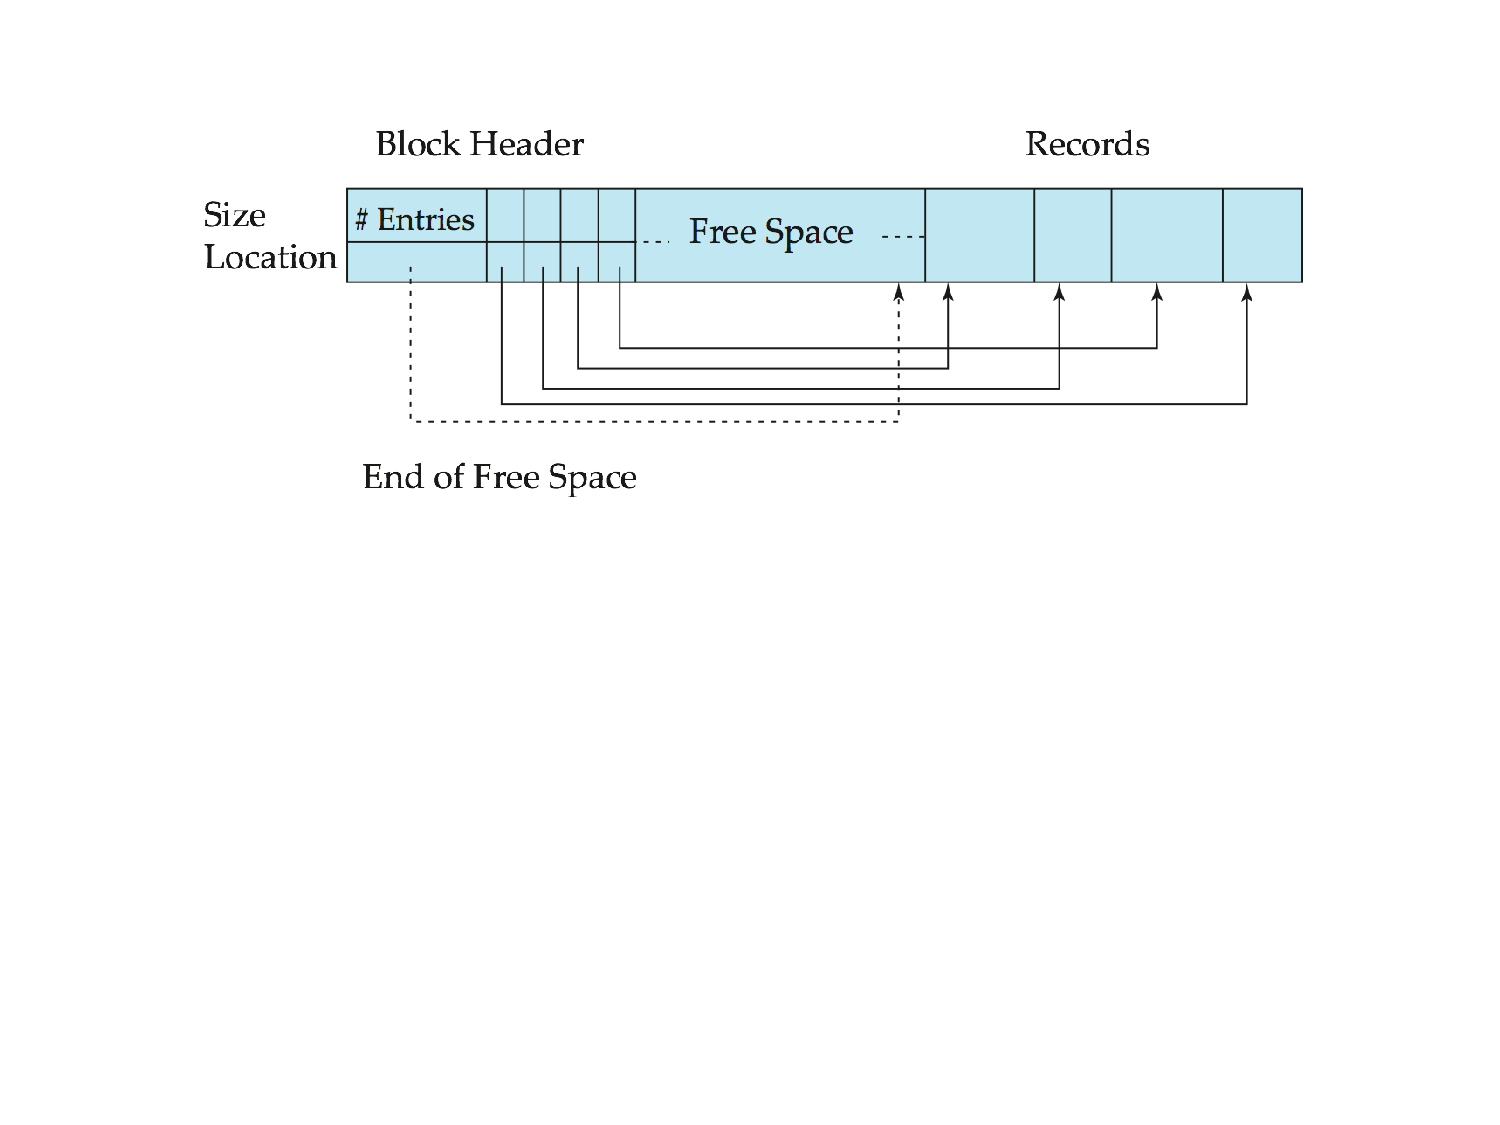
\includegraphics[width=0.8\textwidth]{aula06-slotted}
\caption{Estrutura do \emph{slotted-page}.}
\label{aula06:fig:slotted}
\end{figure}
O cabeçalho contém:
\begin{itemize}
\item número de registros.
\item localização e tamanho de cada registro.
\item fim do espaço livre no bloco.
\end{itemize}
Os registros podem ser movidos dentro de uma página para evitar espaços vazios
entre eles; as entradas no cabeçalho precisam ser atualizadas.
Ponteiros não apontam diretamente para o registro, mas apontam 
para o ponteiro de entrada do registro no cabeçalho.

Registros de tamanho variável aparecem em bancos de dados de diversas formas:
armazenameto de múltiplos tipos de conteúdo em um mesmo arquivo;
armazenamento de atributos que possuem tamanho variável.

Se as slotted-pages são do tamanho de um bloco, o problema dos registros que cruzam é eliminado.
Isso limita o tamanho dos registros em um banco de dados, o que é o caso padrão.

%%%%%%%%%%%%%%%%%%%%%%%%%%%%%%%%%%%%%%%%%%%%%%%%%%%%%%%%%%%%%%%%%%%%%%%%%%%%%%%
\section{Organização de registros em arquivos}
%%%%%%%%%%%%%%%%%%%%%%%%%%%%%%%%%%%%%%%%%%%%%%%%%%%%%%%%%%%%%%%%%%%%%%%%%%%%%%%

Até agora, vimos como representar registros em uma estrutura de arquivo.
Há várias formas de organizar registros em arquivos:
\begin{description}
\item[Heap] um registro pode ser posicionado em qualquer lugar onde haja espaço.

\item[Sequencial] registros armazenados em ordem sequencial, com base
no valor da chave de busca de cada registro.

\item[Hashing] um função hash calculada com base em alguns atributos do 
registro. O resultado especifica em que bloco do arquivo do registro
deve ser posicionado.
\end{description}

%%%%%%%%%%%%%%%%%%%%%%%%%%%%%%%%%%%%%%%%%%%%%%%%%%%%%%%%%%%%%%%%%%%%%%%%%%%%%%%
\subsection{Organização de arquivos sequencial}

Adequada para aplicações que executam processamento sequencial sobre todo o arquivo.
Os registros do arquivo são ordenados por uma \textbf{chave de busca}.

A operação de remoção usa \emph{free lists} para registros de tamanho fixo.

A inserção localiza a posição onde o registro deve ser inserido e:
\begin{enumerate}
\item se houver espaço no bloco, insere no bloco.
\item se for o último registro, insere em um novo bloco.
\item se houver espaço em um bloco vizinho, distribuir. Caso contrário,
insere em um novo \textbf{bloco de estouro} (\emph{overflow block}).
\item de qualquer forma, as cadeias de ponteiros precisam ser atualizadas.
\end{enumerate}
O uso de blocos de estouro demanda a reorganização do arquivo de tempo em tempo
para restaurar a ordem sequencial.

%%%%%%%%%%%%%%%%%%%%%%%%%%%%%%%%%%%%%%%%%%%%%%%%%%%%%%%%%%%%%%%%%%%%%%%%%%%%%%%
\subsection{Clusterização multitable}

Os registros de cada tabela podem ser armazenados em arquivos separados.
Em uma \textbf{clusterização multitable}, registros de tabelas diferentes são armazenados no mesmo 
arquivo.
A principal motivação para armazenar registros relacionados no mesmo bloco é minimizar
a entrada e saída.
A figura~\ref{aula06:fig:clustering1} ilustra a organização de um arquivo com clusterização.
Esse arquivo armazena registros de uma ou mais relações em cada bloco.
Tal organização permite a leitura de registros que podem satisfazer uma união por meio de 
uma leitura de bloco.
%
\begin{figure}[!htb]
\centering
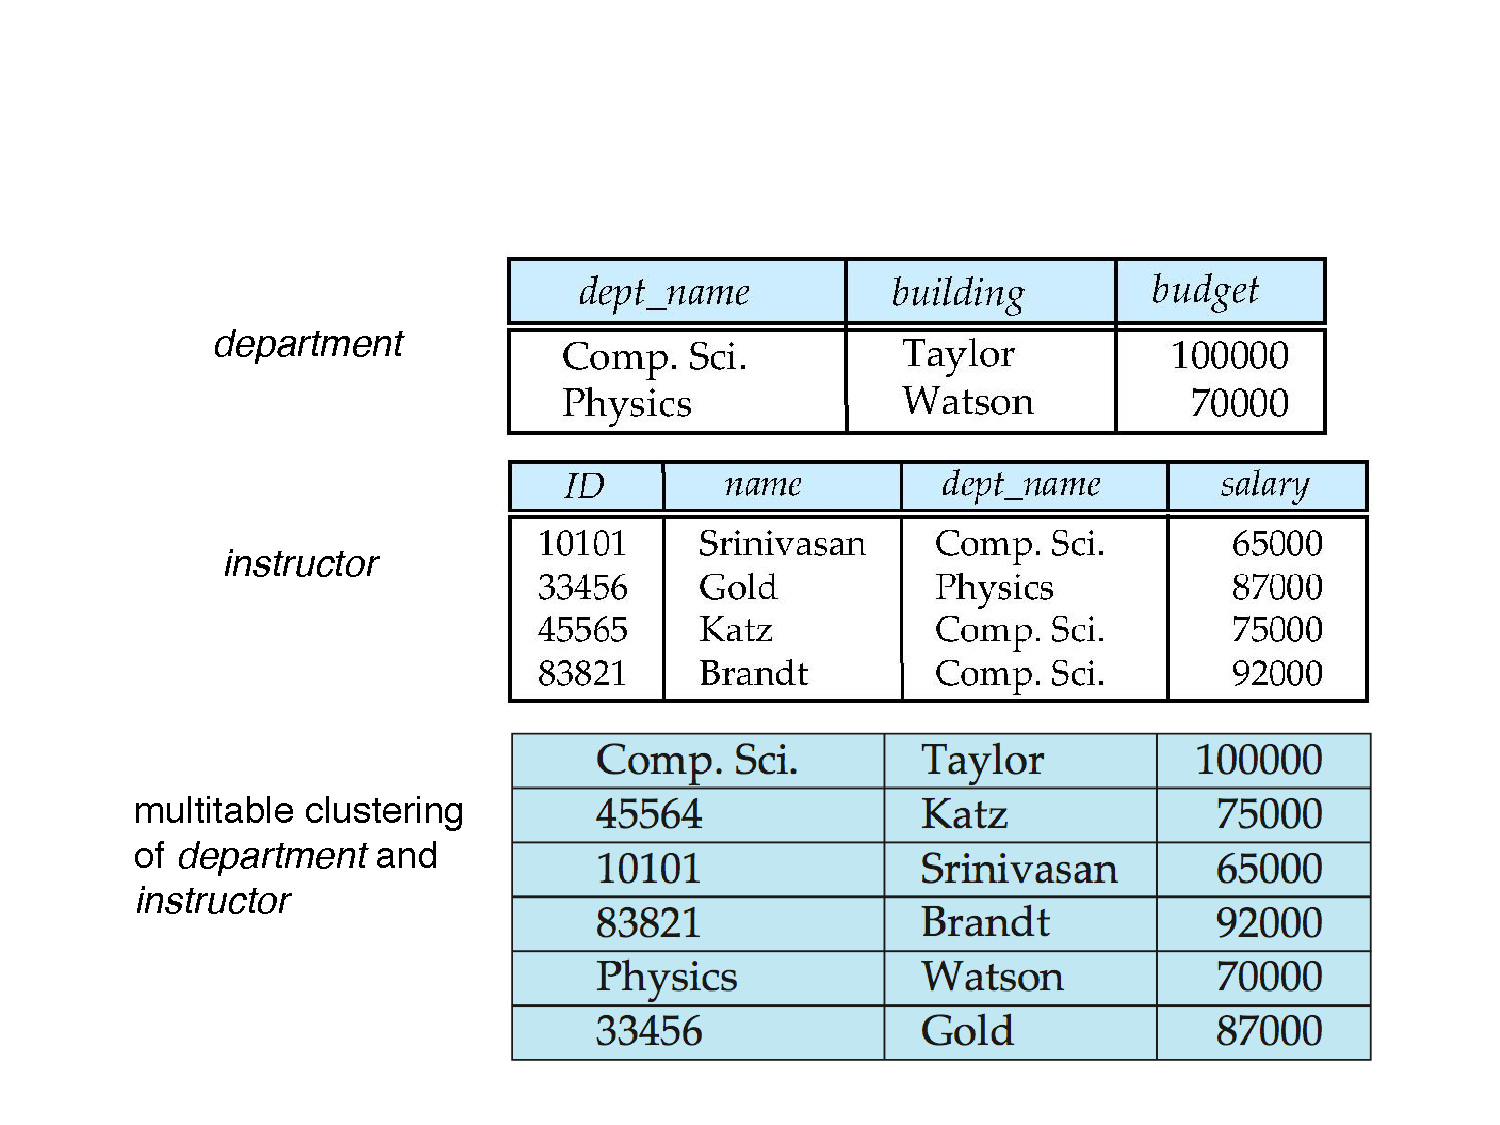
\includegraphics[width=0.6\textwidth]{aula06-clustering1}
\caption{Estrutura de arquivo de uma clusterização multitable.}
\label{aula06:fig:clustering1}
\end{figure}

Essa organização é boa para consultas com relação, e consultas envolvendo um único
deparamento e seus professores.
Porém, ela é ruim para consultas somente de departamentos.

%%%%%%%%%%%%%%%%%%%%%%%%%%%%%%%%%%%%%%%%%%%%%%%%%%%%%%%%%%%%%%%%%%%%%%%%%%%%%%%
\section{Sistemas de arquivos}
%%%%%%%%%%%%%%%%%%%%%%%%%%%%%%%%%%%%%%%%%%%%%%%%%%%%%%%%%%%%%%%%%%%%%%%%%%%%%%%

Em organizações de arquivos sequencias, cada tabela é armazenada em um arquivo.
O armazenamento poderia ser feito por meio do sistema de arquivos do sistema
operacional (SO).
A clusterização multitable pode trazer ganhos significativos em eficiência, mas 
essa organização não é compatível com o sistema de arquivos de sistemas operacionais.

Muitos dos sistemas de bancos de dados (SGBDs) de grande escala não utilizam diretamente o SO.
As tabelas são armazenadas em um único arquivo, e o SGBD gerencia o arquivos por conta própria.
Isso exige a implementação de um sistema de arquivos dentro do SGBD.

%%%%%%%%%%%%%%%%%%%%%%%%%%%%%%%%%%%%%%%%%%%%%%%%%%%%%%%%%%%%%%%%%%%%%%%%%%%%%%%
\subsection{Buffer manager}

O  número de transferencias de blocos entre o disco e a memória pode ser
reduzido mantendo o maior número possível de blocos na memória principal.
Um \textbf{buffer} é a porção da memória principal disponível para armazenar cópias
de blocos de disco.
O \textbf{buffer manager} é responsável pela alocação de espaço do buffer na 
memória principal.

Programas utilizam o buffer manager quando precisam ler um bloco do disco:
\begin{enumerate}
\item se o bloco já estiver no buffer, o gerenciador retorna o endereço 
do bloco na memória principal.

\item se o bloco não estiver no buffer, o manager:
	\begin{enumerate}
	\item aloca espaço no buffer para o bloco.
		\begin{enumerate}
		\item substituindo algum outro bloco, se necessário, para
			liberar espaço para o novo bloco.
		\item o bloco substituído é escrito de volta no disco somente se ele foi
		modificado desde a última vez que ele foi escrito/recuperado do disco.
		\end{enumerate}
	\item Lê o bloco do disco para o buffer e retorna o endereço do bloco
		na memóra principal para o programa.
	\end{enumerate}
\end{enumerate}

Sua função é similar ao gerenciamento e memória virtual dos sistemas operacionais.
Porém, bancos de dados tem requisitos diferentes.

%%%%%%%%%%%%%%%%%%%%%%%%%%%%%%%%%%%%%%%%%%%%%%%%%%%%%%%%%%%%%%%%%%%%%%%%%%%%%%%
\subsection{Políticas de substituição de blocos}

A maioria dos sistemas operacionais usam a política de substituição do bloco menos recentemente usado
ou \emph{least recently used} (LRU).
A ideia por trás do LRU é usar um padrão passado de referência a blocos como uma previsão de 
futuras referências, já que usualmente nada mais se conhece.
Consultas possuem um padrão de acesso bem definido, com varreduras sequenciais.
O sistema do BD pode usar informação contida na consulta para prever referências futuras.

O LRU pode ser uma estratégia ruim para certos tipos de acesso que envolvem varreduras repetidas.
Por exemplo, na junção de 2 tabelas $r$ e $s$ por um laço aninhado. 
Uma estratégia mista é preferível, onde o otimizador de consultas pode oferecer dicas
para substituição de blocos.

Outras técnicas do buffer manager são:
\begin{description}
\item[Pinned block] bloco em memória que não tem permissão de ser escrito
de volta no disco.

\item[Estratégia Toss-immediate]  libera o espaço ocupado por um bloco assim que 
a última tupla do bloco é processada.

\item[Estratégia MRU] MRU significa mais recentemente usado (\emph{most recently used}), onde 
o sistema marca o bloco sendo processado. Depois que a última tupla do bloco é processada,
o bloco é desmarcado, e se torna o bloco mais recentemente usado.

\item[Saída forçada] o manager também suporta saída forçada de blocos para fins de 
recuperação.
\end{description}

%%%%%%%%%%%%%%%%%%%%%%%%%%%%%%%%%%%%%%%%%%%%%%%%%%%%%%%%%%%%%%%%%%%%%%%%%%%%%%%
\section{Mecanismos de indexação}
%%%%%%%%%%%%%%%%%%%%%%%%%%%%%%%%%%%%%%%%%%%%%%%%%%%%%%%%%%%%%%%%%%%%%%%%%%%%%%%

Muitas buscas referenciam apenas uma pequena porção dos registros de um arquivo.
Seria ineficiente ler todos os registros para encontrar apenas uma tupla.
Usa-se estruturas adicionais a fim de permitir esse tipo de acesso.

%%%%%%%%%%%%%%%%%%%%%%%%%%%%%%%%%%%%%%%%%%%%%%%%%%%%%%%%%%%%%%%%%%%%%%%%%%%%%%%
\subsection{Introdução}

Um índice de um arquivo funciona como o índice de um livro.
Mecanismos de indexação são utilizados para acelerar o acesso
aos dados.
Uma \textbf{chave de busca} (\emph{search key}) é/são o(s) atributo(s) usado(s)
para localizar registros em um arquivo.
Um \textbf{arquivo de índice} consiste em registros na forma \emph{chave -
pointeiro}.
Arquivos de índice são muito menores que o arquivo original.

Há dois tipos básicos de índices:
\begin{description}
\item[Índices ordenados] chaves de busca são armazenadas (encadeadas) em ordem.
\item[Índices hash]  chaves de busca são distribuídas uniformemente
em buckets usando uma função de hash.
\end{description}

As duas técnicas são estudadas. 
Nenhuma delas é considerada a melhor. 
Cada técnica é avaliada de acordo com os seguintes fatores:
\begin{description}
\item[Tipo de acesso eficiente]  como registros de um valor específico em um atributo. Esse fator
exerce bastante influência na escolha do tipo de índice.
\item[Tempo de acesso]
\item[Tempo de inserção]
\item[Tempo de remoção]
\item[Sobrecarga de espaço] sendo o espaço adicional para o índice.
\end{description}

%%%%%%%%%%%%%%%%%%%%%%%%%%%%%%%%%%%%%%%%%%%%%%%%%%%%%%%%%%%%%%%%%%%%%%%%%%%%%%%
\subsection{Índices ordenados}

Em um \textbf{índice ordenado}, as entradas são ordenadas de acordo
com o valor da chave de busca, como por exemplo pelo nome do autor em um catálogo.
Podem ser classificados quanto:
\begin{itemize}
\item A chave de busca indexada.
	\begin{itemize}
	\item índices primários.
	\item índices secundários.
	\end{itemize}
\item Aos registros indexados.
	\begin{itemize}
	\item índices densos.
	\item índices esparsos.
	\end{itemize}
\end{itemize}

O \textbf{índice primário}, em um arquivo sequencialmente ordenado, é o índice
cuja chave de busca é usada para ordenar o arquivo.
É também chamado de \textbf{índice clusterizado} (\emph{clustering index}).
A chave de busca de um índice primário é quase sempre a chave primária.

O \textbf{índice secundário} é um índice cuja chave de busca não está armazenada
de acordo com a ordem sequencial do arquivo.
Também chamado de \textbf{índice não clusterizado} (\emph{non-clustering index}).

%%%%%%%%%%%%%%%%%%%%%%%%%%%%%%%%%%%%%%%%%%%%%%%%%%%%%%%%%%%%%%%%%%%%%%%%%%%%%%%
\subsection{Índices densos e esparsos}

Uma entrada no índice consiste em uma chave de busca e pointeiros para um ou mais registros.
O ponteiro para um registro consiste no identificador de um bloco do disco e um deslocamento
dentro do bloco para identificar o registro.
Há dois tipos de índices: denso e esparso.

\textbf{Índices esparsos} contém entradas no índice para apenas alguns valores de chave de busca.
Para localizar um registro com uma chave de busca $k$, deve-se:
\begin{enumerate}
\item encontrar a entrada com o maior valor de chave de busca $< k$.
\item varrer o arquivo sequencialmente a partir do resgistro apontado por essa entrada.
\end{enumerate}
Índices esparsos são somente aplicáveis quando os registros estão ordenados pela chave
de busca do índice.

Em \textbf{índices densos} registros do índice aparecem para todos os valores
de chave de busca do arquivo.
Índices primários podem ser densos ou esparsos, mas índices secundários
precisam ser densos.

A figura~\ref{aula06:fig:denso:esparso} ilustra um exemplo entre índices denso e esparso.
%
\begin{figure}[!htb]
\centering
  \begin{minipage}{0.45\textwidth}
	\centering
	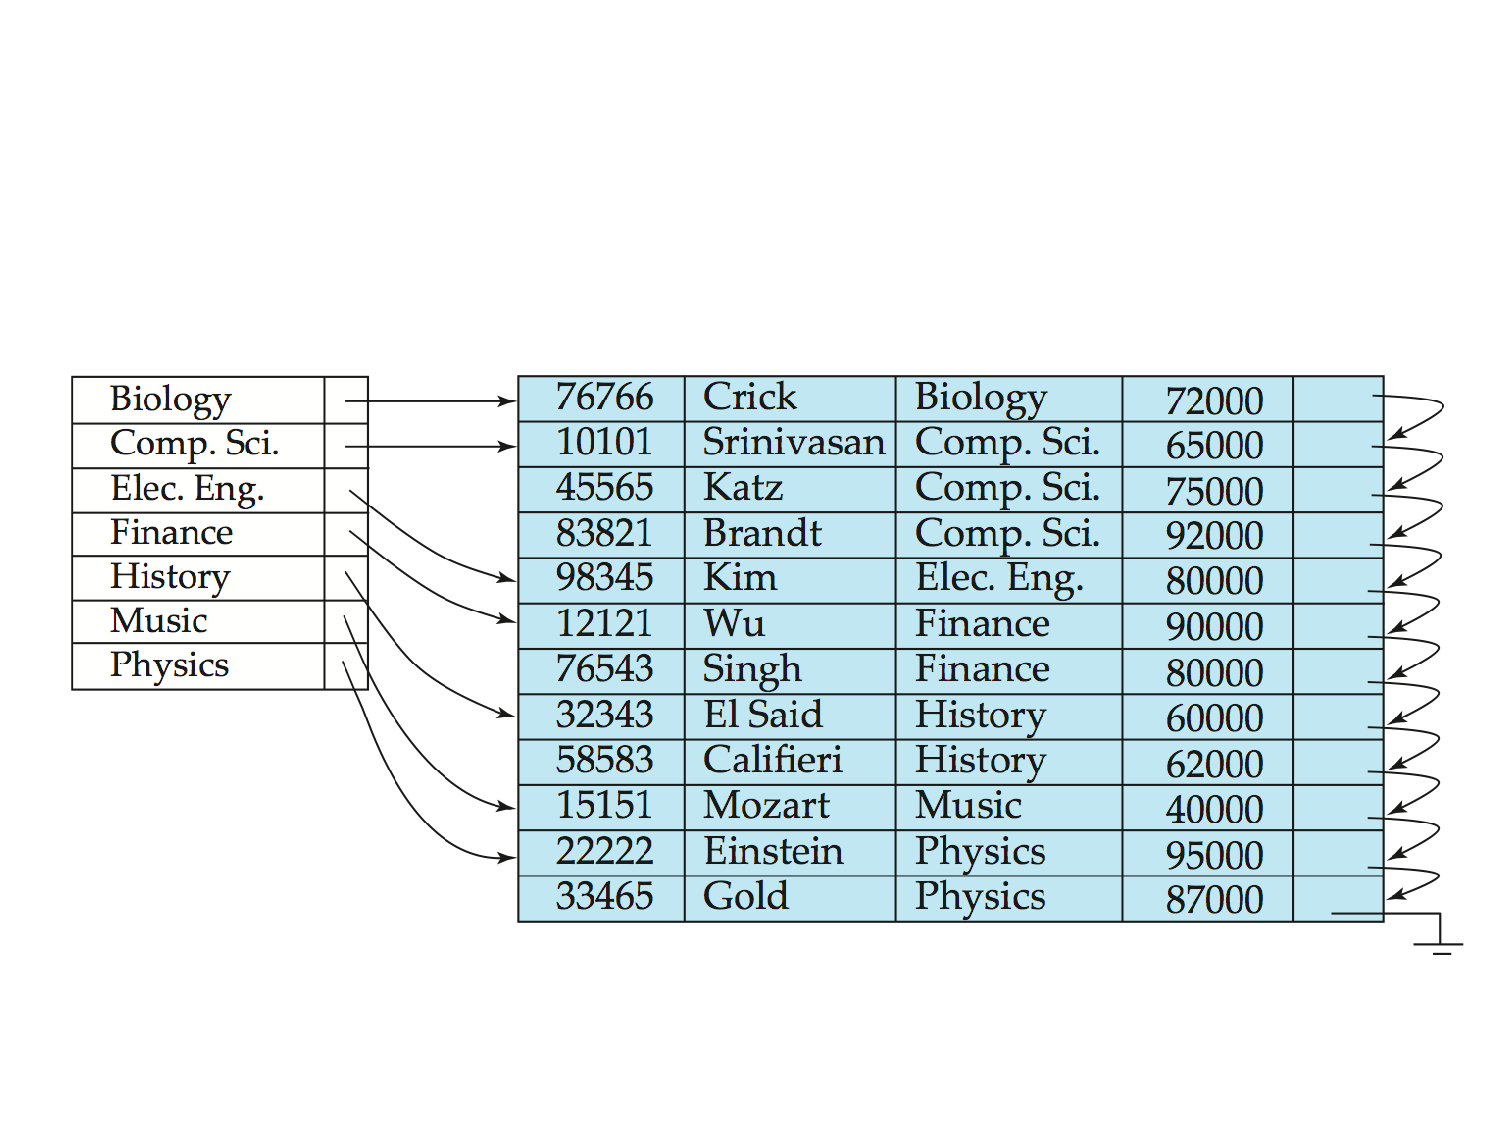
\includegraphics[width=\textwidth]{aula06-denso1}
  \end{minipage}
  %
  \begin{minipage}{0.45\textwidth}
	\centering
	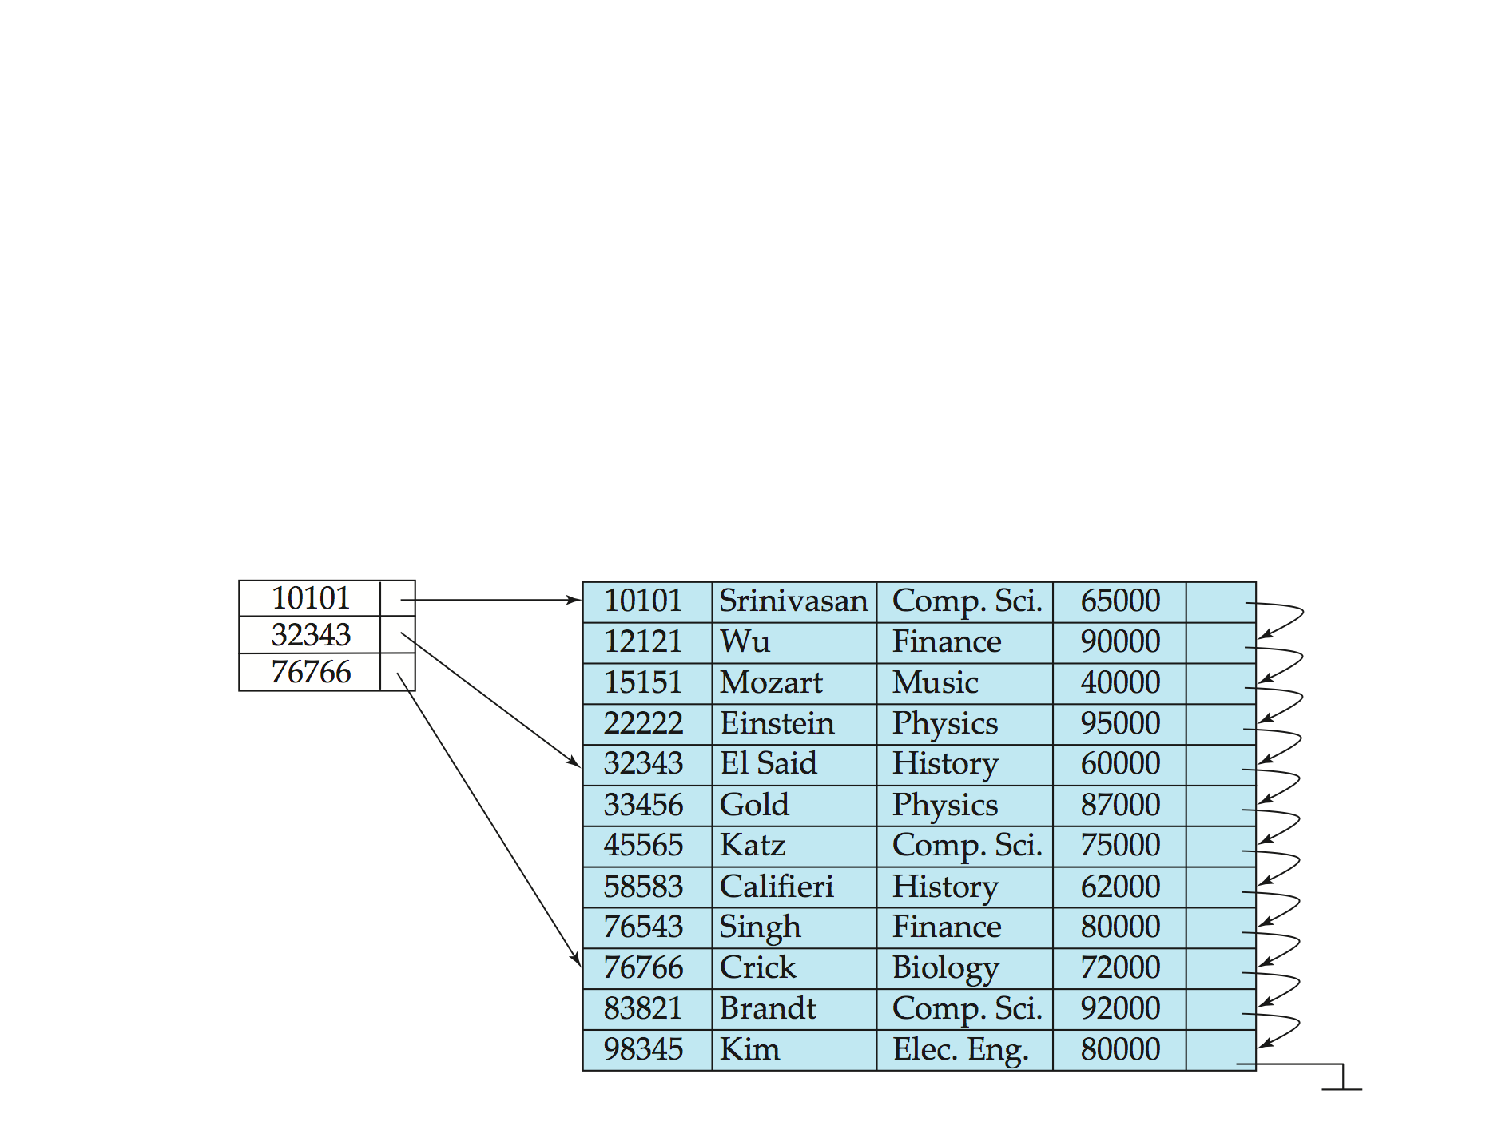
\includegraphics[width=\textwidth]{aula06-esparso1}
  \end{minipage}
\caption{Exemplo de um índice denso (esquerda) e esparso (direita).}
\label{aula06:fig:denso:esparso}
\end{figure}

%%%%%%%%%%%%%%%%%%%%%%%%%%%%%%%%%%%%%%%%%%%%%%%%%%%%%%%%%%%%%%%%%%%%%%%%%%%%%%%
\subsection{Índices multinível}

Para casos em que o índice primário não cabe em memória, o acesso torna-se caro.
Uma solução é tratar o índice primário em disco como um arquivo sequencial e
construir um índice esparso sobre ele.
O \textbf{índice externo} é um índice esparso do índice primário, e 
o \textbf{índice interno} é o arquivo do índice primário.

Se mesmo o índice externo for muito grande para caber na memória, outro nível
pode ser criado, e assim por diante.
Note que índices em todos os níveis devem ser atualizados quando ocorrer
atualizações no arquivo.
A figura~\ref{aula06:fig:multinivel} mostra um simples exemplo de índice esparso
construído de um índice primário.
%
\begin{figure}[!htb]
\centering
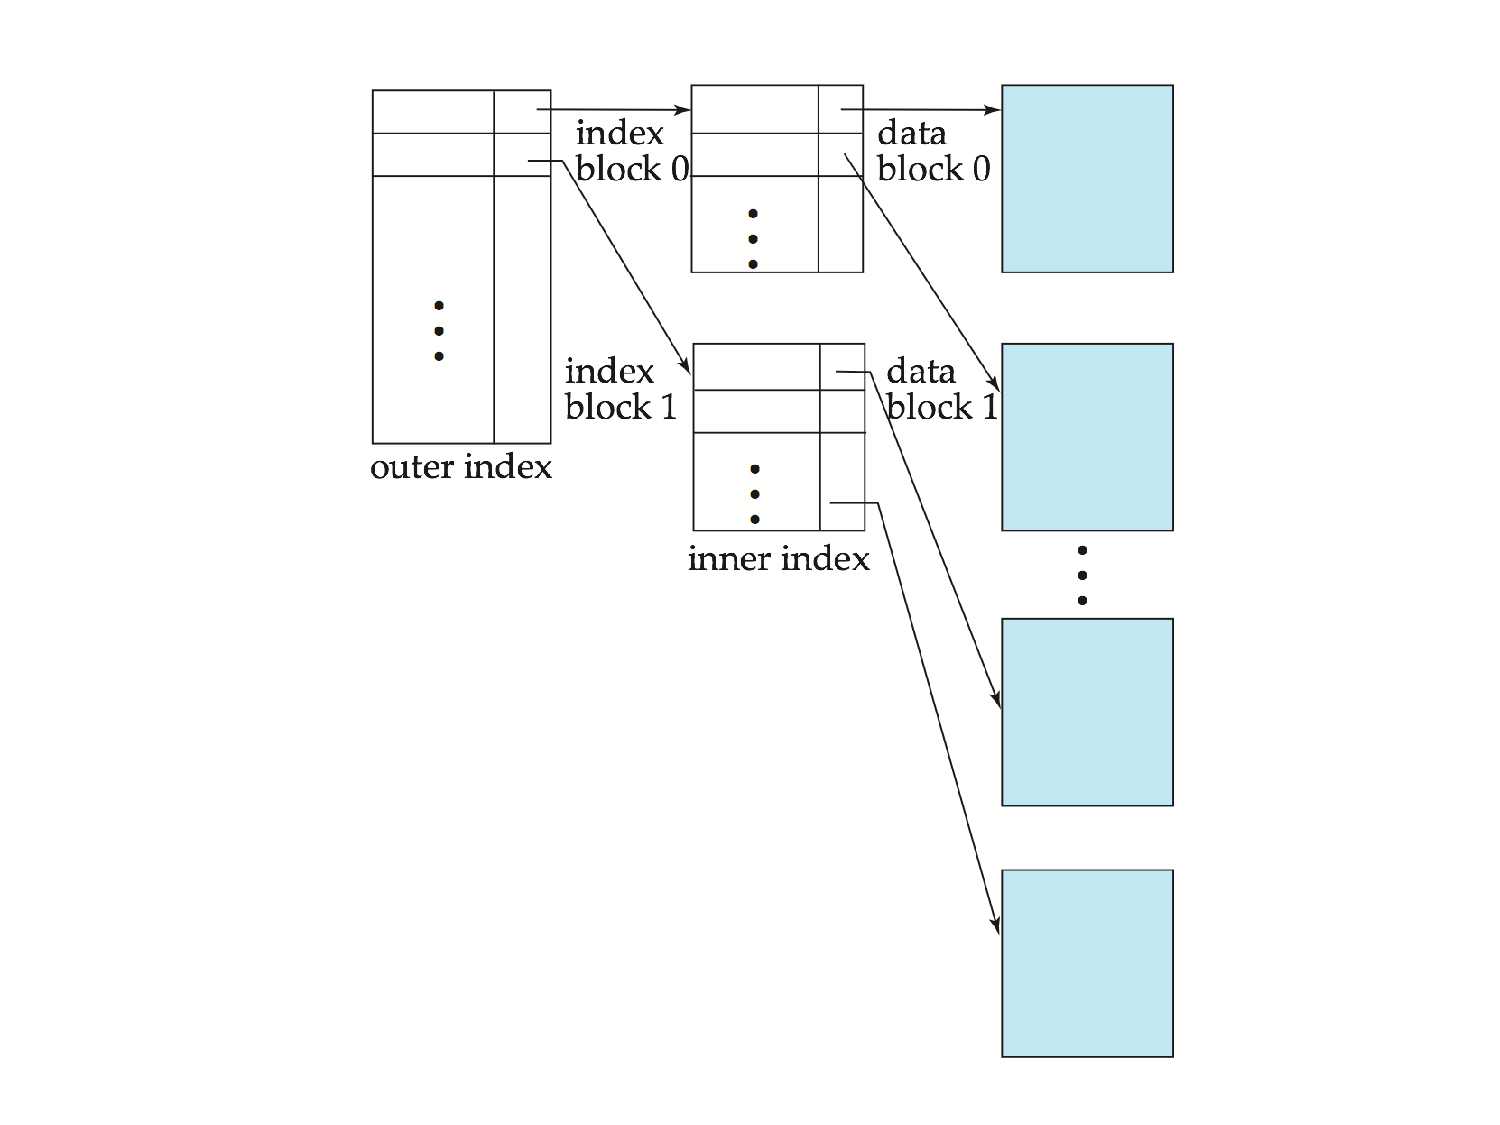
\includegraphics[width=0.4\textwidth]{aula06-multinivel1}
\caption{Índice esparso externo construído de um índice primário.}
\label{aula06:fig:multinivel}
\end{figure}

%%%%%%%%%%%%%%%%%%%%%%%%%%%%%%%%%%%%%%%%%%%%%%%%%%%%%%%%%%%%%%%%%%%%%%%%%%%%%%%
\subsection{Atualização de índice}

Em qualquer das formas de índice, cada índice precisa ser atualizado quando um
registro é inserido ou removido.

{\bf Remoção} - se o registro removido é o único registro no arquivo
com uma chave de busca, a chave de busca também é removida do índice.
Em índices densos, remoção de uma chave de busca é similar a remoção
de um registro de arquivo.
Em índices esparsos, se uma chave de busca existe no índice, ela é removida 
e substituída pela próxima chave de busca do arquivo.
Se a próxima chave de busca já for indexada, a entrada no índice é simplesmente 
removida.

{\bf Inserção} - em índíces densos, realiza uma busca no índice usando a chave de
busca do registro a ser inserido.
Se a chave não existe, ela é inserida no índice.
Em índices esparsos, se o índice mantem uma entrada para cada bloco do arquivo,
nenhuma mudança é necessária, a não ser que um novo bloco seja criado (ou sofra
distribuição).
Se um novo bloco for criado (ou sofrer distribuição), 
a primeira chave de busca nova do bloco é inserida no índice.

Em índices multinível, as inserções e remoções são simples extensões dos
algoritmos usados em índices de um nível só.
As inserções e remoções são propagadas dos níveis internos para os externos.

As atualizações dos índices significam atualizações nos blocos físicos
onde os índices estão armazenados.
A organização física e lógica desses blocos é feita de forma similar
aos blocos de um arquivo de dados.

%%%%%%%%%%%%%%%%%%%%%%%%%%%%%%%%%%%%%%%%%%%%%%%%%%%%%%%%%%%%%%%%%%%%%%%%%%%%%%%
\subsection{Índices secundários}

Em índices secundários, registros do índice apontam para o bucket que contem pointeiros
para todos os registros com uma chave de busca.
A figura~\ref{aula06:fig:secundario} mostra um exemplo de índice secundário.
Note que índices secundários tem de ser densos.
%
\begin{figure}[!htb]
\centering
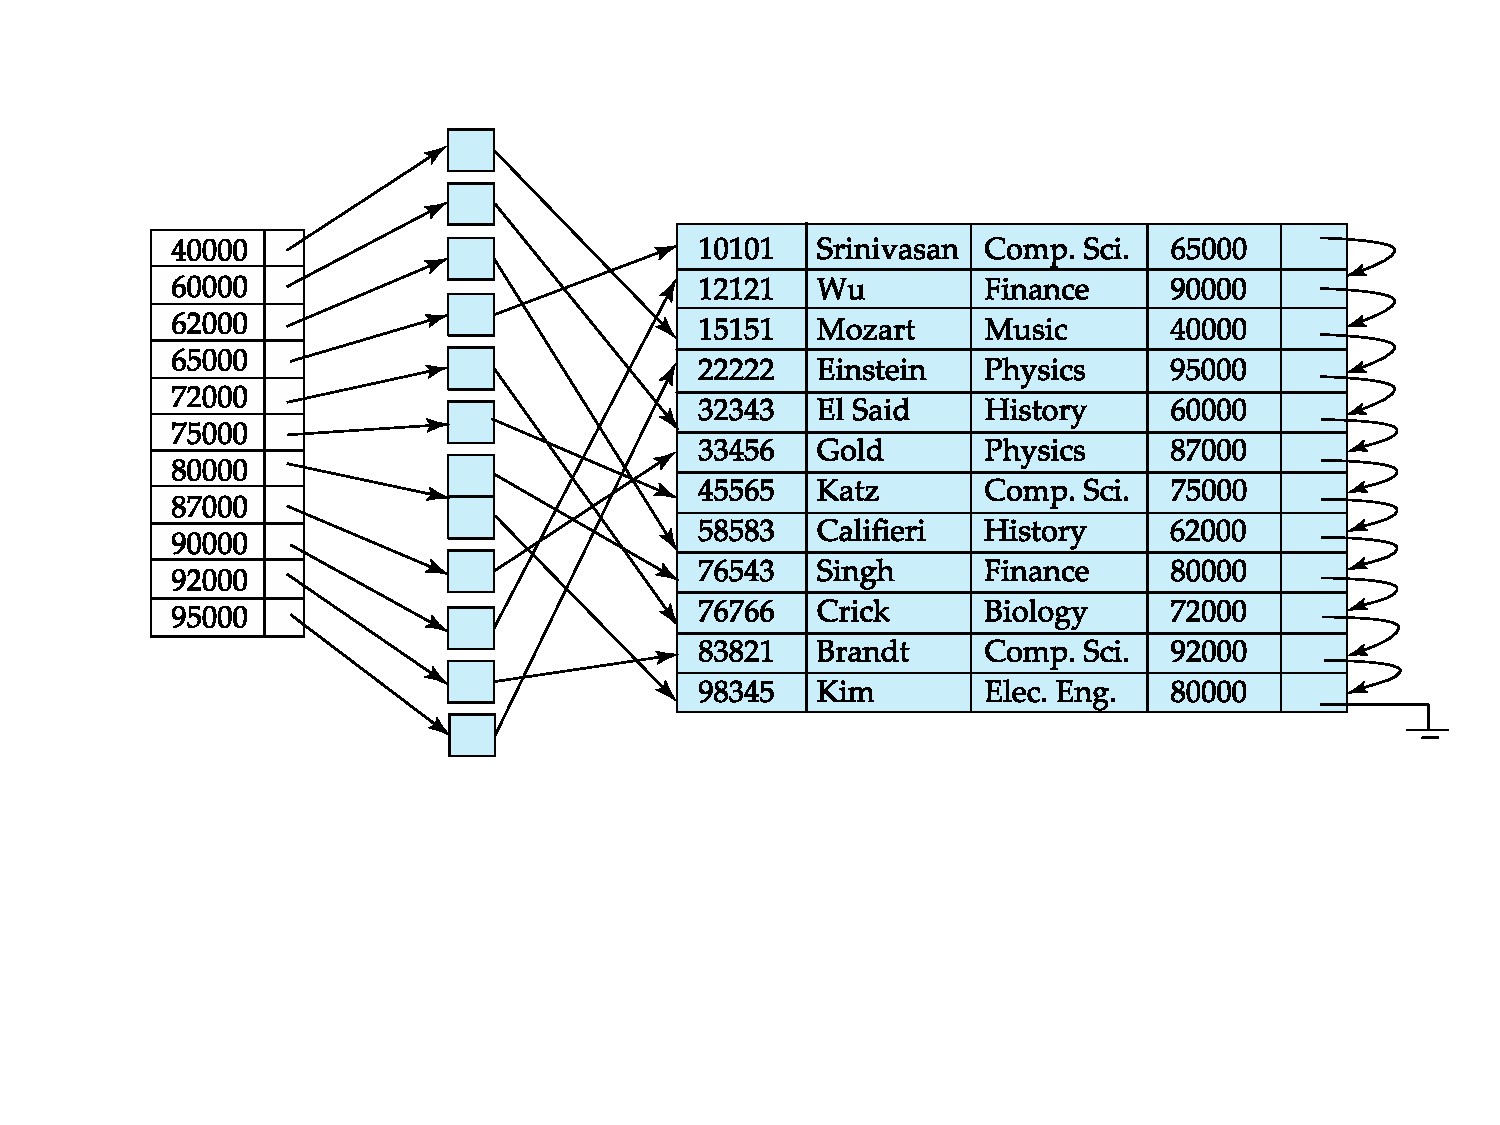
\includegraphics[width=0.6\textwidth]{aula06-secundario1}
\caption{Exemplo de índice secundário sobre o campo \emph{salary}.}
\label{aula06:fig:secundario}
\end{figure}

Índices oferecem benefícios substanciais na busca por registros.
Porém, atualizações de índices impõem sobrecustos em atualizações.

A varredura sequencial de um índice primário é eficiente, mas a 
varredura sequencial em índices secundários é cara pois é preciso
uma transferência de bloco do disco para cada acesso ao registro.
Uma transferência de bloco requer cerca de 5 a 10 milisegundos, contra
100 nanosegundos de um acesso à memória.

%%%%%%%%%%%%%%%%%%%%%%%%%%%%%%%%%%%%%%%%%%%%%%%%%%%%%%%%%%%%%%%%%%%%%%%%%%%%%%%
%\subsection{conceitos basicos}

%%%%%%%%%%%%%%%%%%%%%%%%%%%%%%%%%%%%%%%%%%%%%%%%%%%%%%%%%%%%%%%%%%%%%%%%%%%%%%%
\section{Índices em árvores B+}
%%%%%%%%%%%%%%%%%%%%%%%%%%%%%%%%%%%%%%%%%%%%%%%%%%%%%%%%%%%%%%%%%%%%%%%%%%%%%%%

A principal desvantagem de índices sequenciais é a perda de desempenho
a medida que o arquivo de índice cresce, tanto buscas e varreduras sequenciais.
Reorganizações periódicas são necessárias, mas reorganizações frequentes
são indesejadas.
\textbf{Índices em árvores B+} é um tipo de árvore balanceada que mantem a eficiência
mesmo com inserções e remoções.
Cada nó não-folha de uma árvore B+ tem entre $\lceil n/2 \rceil$ e $n$ filhos,
sendo $n$ fixo para uma árvore particular.

Árvores B+ tem a vantagem de se auto-organizar com modificações pequenas e
locais em inserções e remoções, além de não requerer a reorganização de todo o
arquivo para manter o desempenho.
Uma desvantagem menor é o sobrecusto de inserção e remoção para manter o 
balanceamento, além do sobrecusto em espaço.

A figura~\ref{aula06:fig:btree1} mostra um exemplo de árvore B+.
%
\begin{figure}[!htb]
\centering
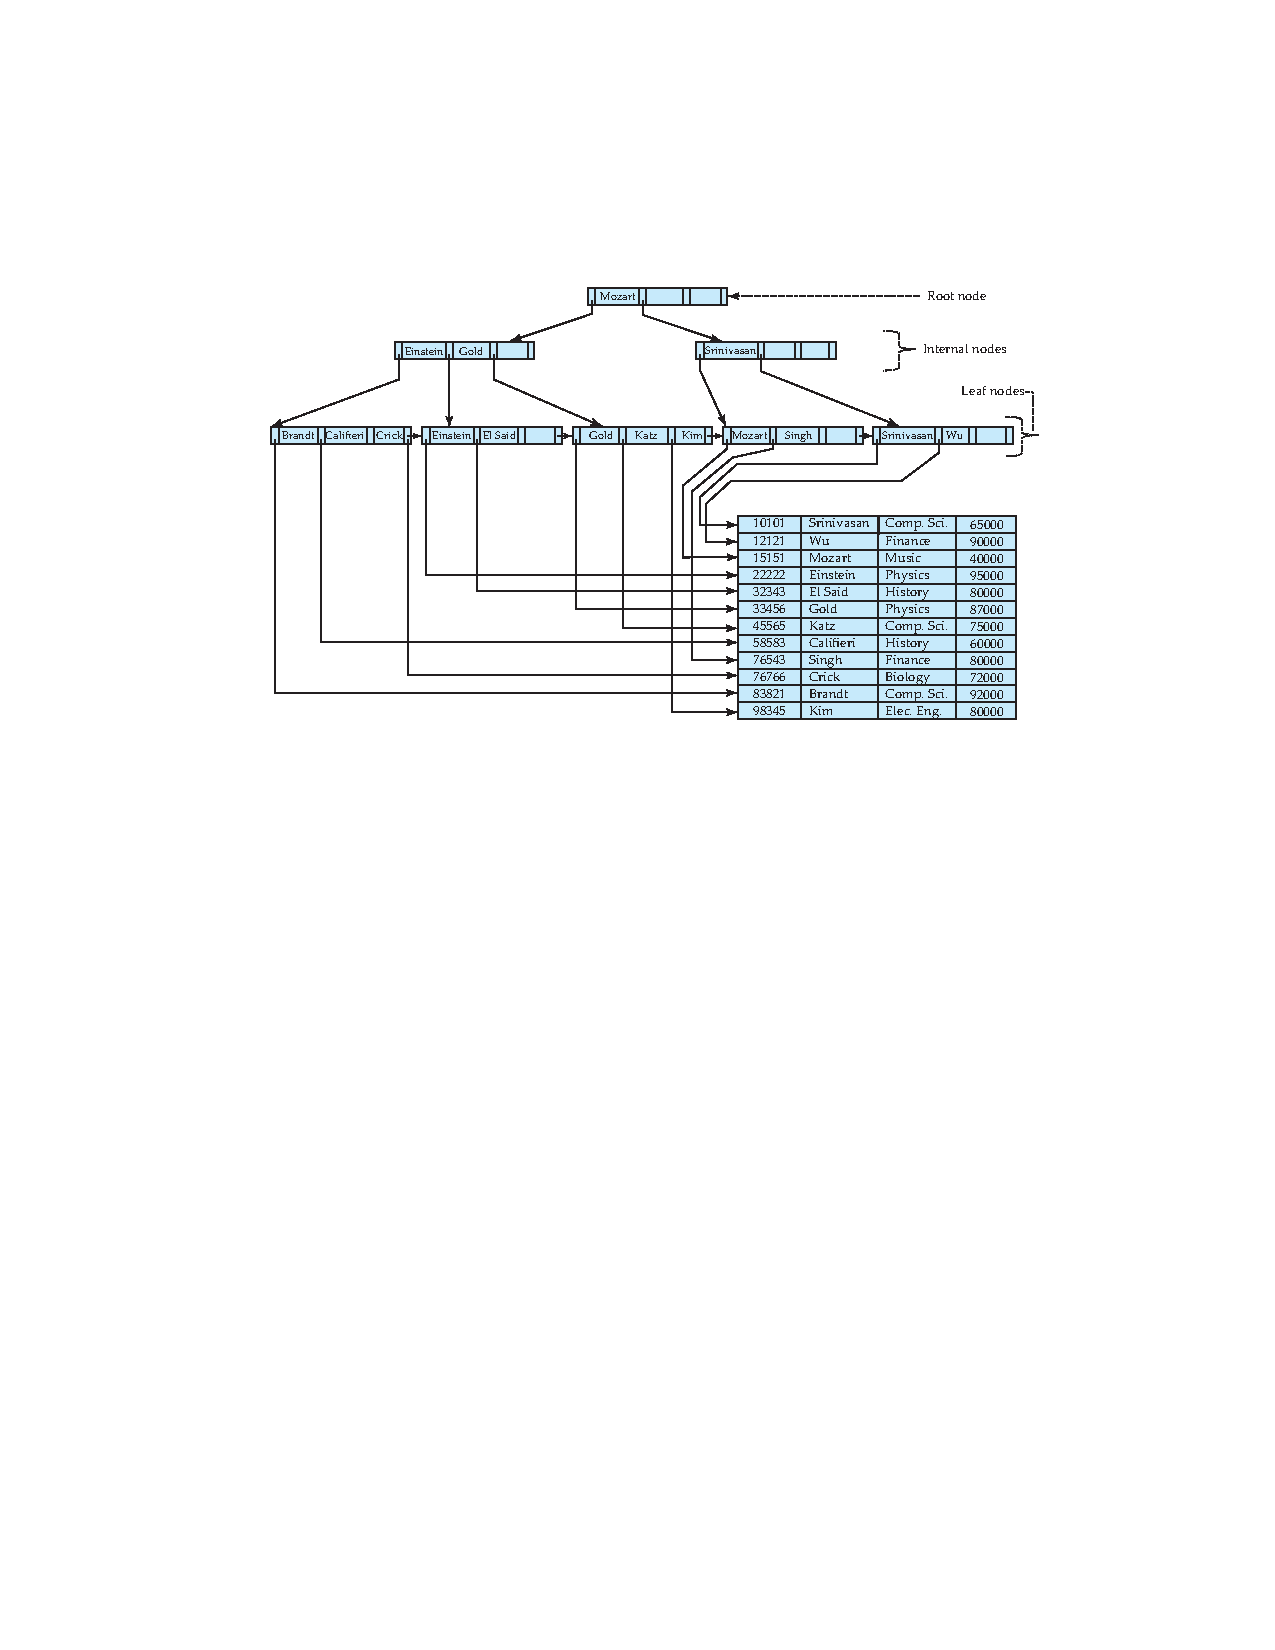
\includegraphics[width=0.7\textwidth]{aula06-btree1}
\caption{Exemplo de uma árvore B+.}
\label{aula06:fig:btree1}
\end{figure}

Uma árvore B+ é uma árvore com raiz única que segue as seguintes propriedades:
\begin{itemize}
\item Todos os caminhos da raiz até as folhas tem o mesmo tamanho.
\item Cada nó que não seja raiz nem folha possui de $\lceil n/2 \rceil$
até $n$ filhos.
\item Um nó folha tem de $\lceil (n-1)/2 \rceil$ até $n-1$ valores.
\item Casos especiais:
	\begin{itemize}
	\item Se a raiz não é uma folha, ela possui pelo menos dois filhos.
	\item Se a raiz é uma folha (ou seja, é o único nó da árvore), ela
	pode ter de $0$ a $(n-1)$ valores.
	\end{itemize}
\end{itemize}

%%%%%%%%%%%%%%%%%%%%%%%%%%%%%%%%%%%%%%%%%%%%%%%%%%%%%%%%%%%%%%%%%%%%%%%%%%%%%%%
\subsection{Estrutura}

Um nó típico de árvore B+, como na figura~\ref{aula06:fig:btree2}, possui:
\begin{itemize}
\item $K_i$ são valores de chaves de busca.
\item $P_i$ são pointeiros para filhos (nós não folha), ou para
registros ou buckets de registros (para nós folha).
\end{itemize}
As chaves de busca de um nó são ordenadas com $K_1 < K_2 < K_3 < ... < K_{n-1}$.
Normalmente o nó tem o tamanho de um bloco.
%
\begin{figure}[!htb]
\centering
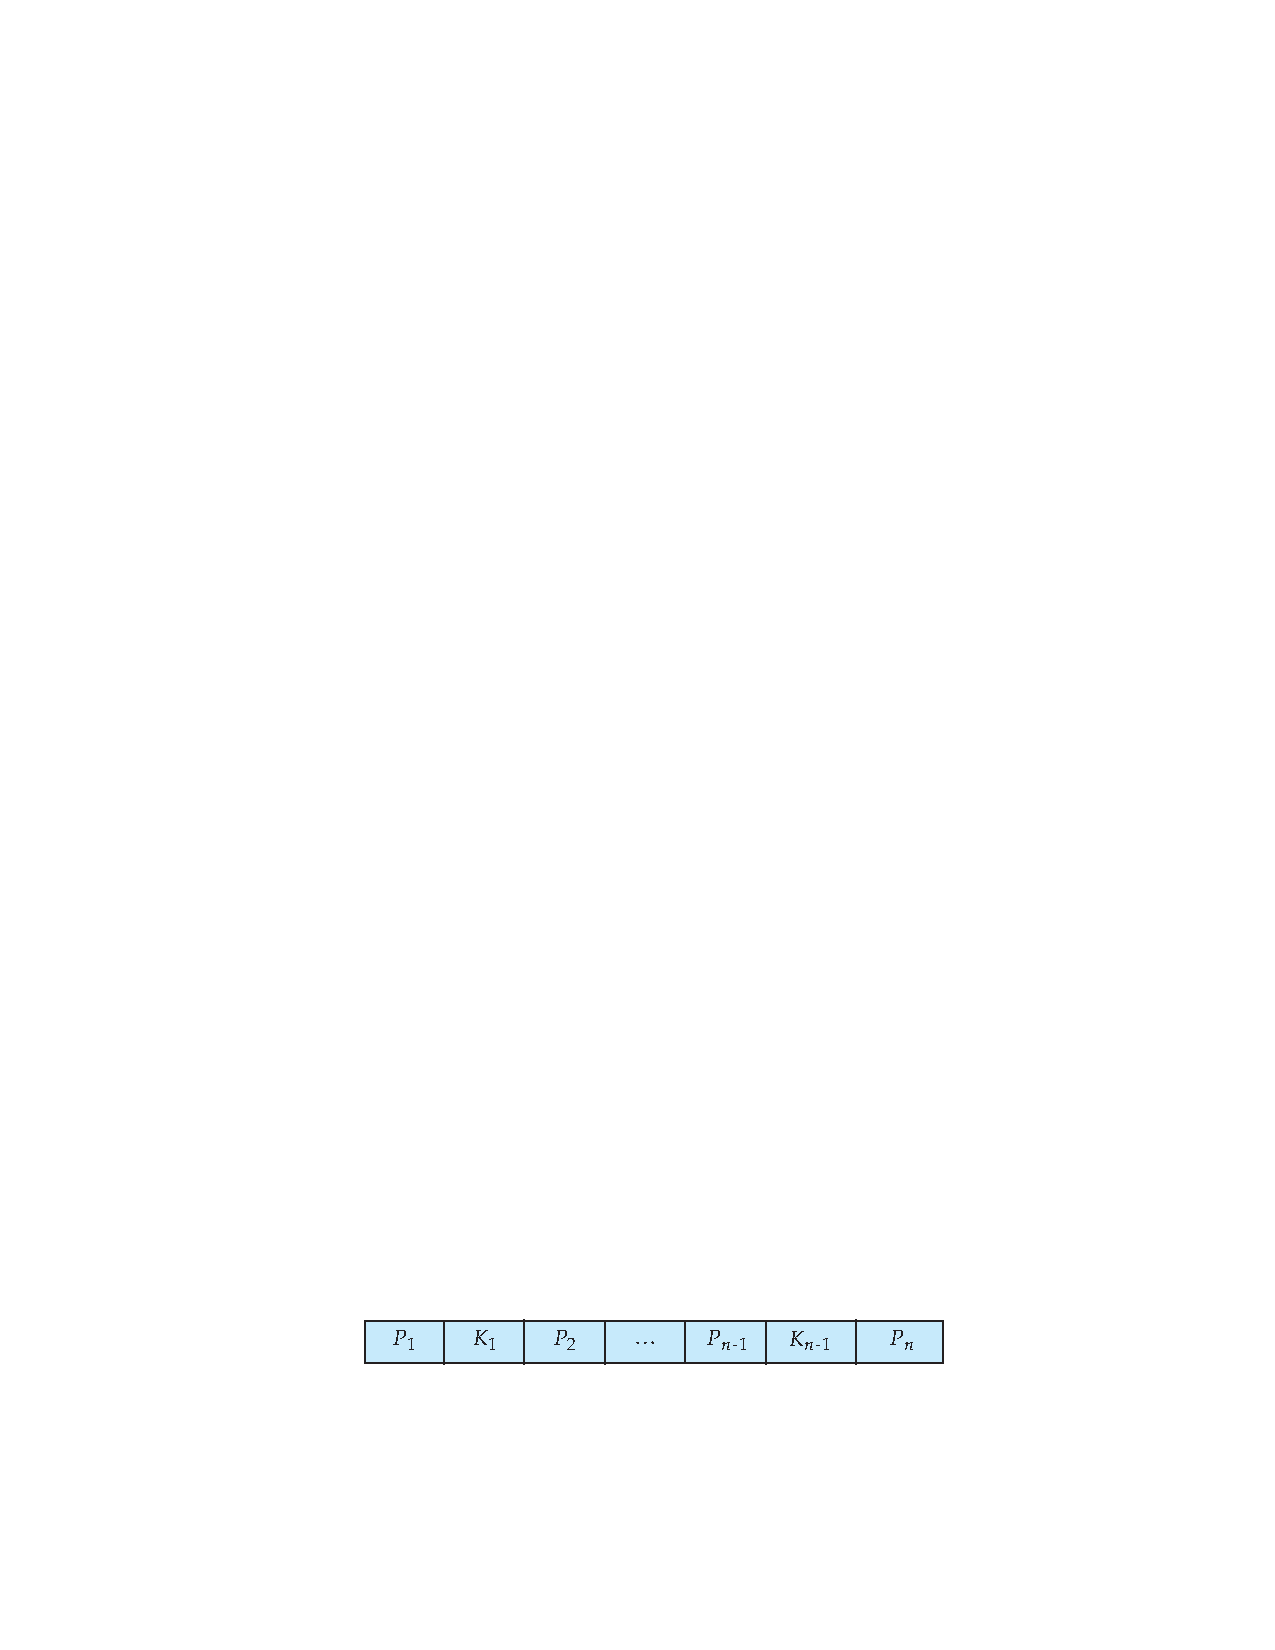
\includegraphics[width=0.4\textwidth]{aula06-btree2}
\caption{Um nó em uma árvore B+.}
\label{aula06:fig:btree2}
\end{figure}

As propriedades de um nó folha, como na figura~\ref{aula06:fig:btree3}, são:
\begin{itemize}
\item Para $i = 1, 2, ..., n-1$, o ponteiro $P_i$ aponta
para o registro com chave de busca $K_i$, ou para um bucket de apontadores para registros.
Buckets só são necessários se a chave de busca não for chave primária.
\item Se $L_i$, $L_j$ são nós folha e $i < j$, as chaves de busca de $L_i$
são menores que as chaves de busca de $L_j$.
\item $P_n$ aponta para o próximo nó folha na ordem da chave de busca.
\end{itemize}
%
\begin{figure}[!htb]
\centering
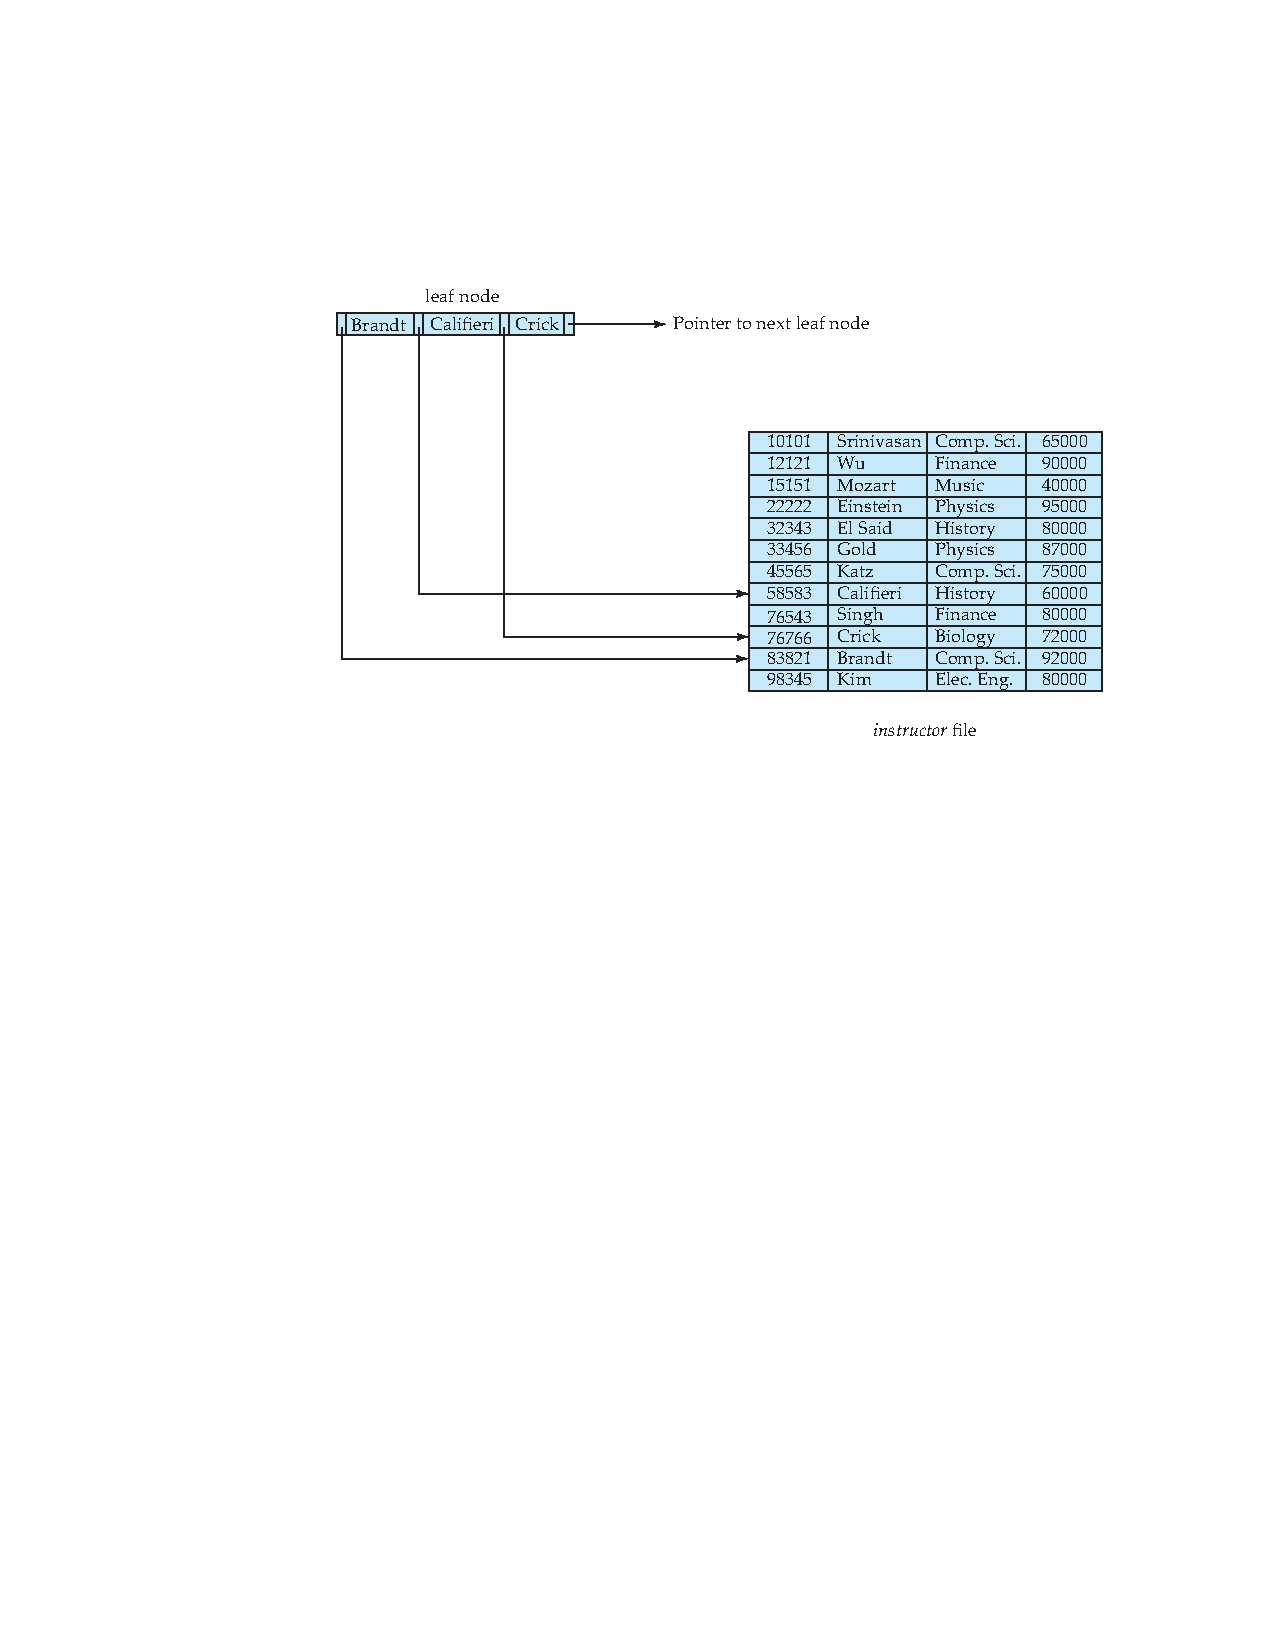
\includegraphics[width=0.6\textwidth]{aula06-btree3}
\caption{Exemplo de um nó folha ($n = 4$) de uma árvore B+.}
\label{aula06:fig:btree3}
\end{figure}

Ao passo que nós não folha formam um índice esparso multinível sobre os nós folha.
Para um nó não folha, como na figura~\ref{aula06:fig:btree2}, com $m$ ponteiros:
\begin{itemize}
\item Todas as chaves de busca da subárvore apontada por $P_1$ são 
menores do que $K_1$.
\item Para $2 \leq i \leq n-1$, todas as chaves de busca da sub-árvore apontada
por $P_i$ são maiores ou iguais a $K_{i-1}$ e menores que $K_i$.
\item Todas as chaves de busca da sub-árvore apontada por $P_n$ são maiores
ou iguais a $K_{n-1}$.
\end{itemize}

A figura~\ref{aula06:fig:btree4} ilustra um exemplo de árvore B+ com $n = 6$.
Baseado nessa figura, podemos afirmar que:
\begin{itemize}
\item Nós folha tem de 3 a 5 valores ($\lceil (n-1)/2 \rceil$ e $n-1$, com $n=6$).
\item Nós não folha (que não a raiz) tem de 3 a 6 filhos ($\lceil n/2 \rceil$ e
$n$ com $n=6$).
\item A raiz precisa ter pelo menos $2$ filhos.
\end{itemize}
%
\begin{figure}[!htb]
\centering
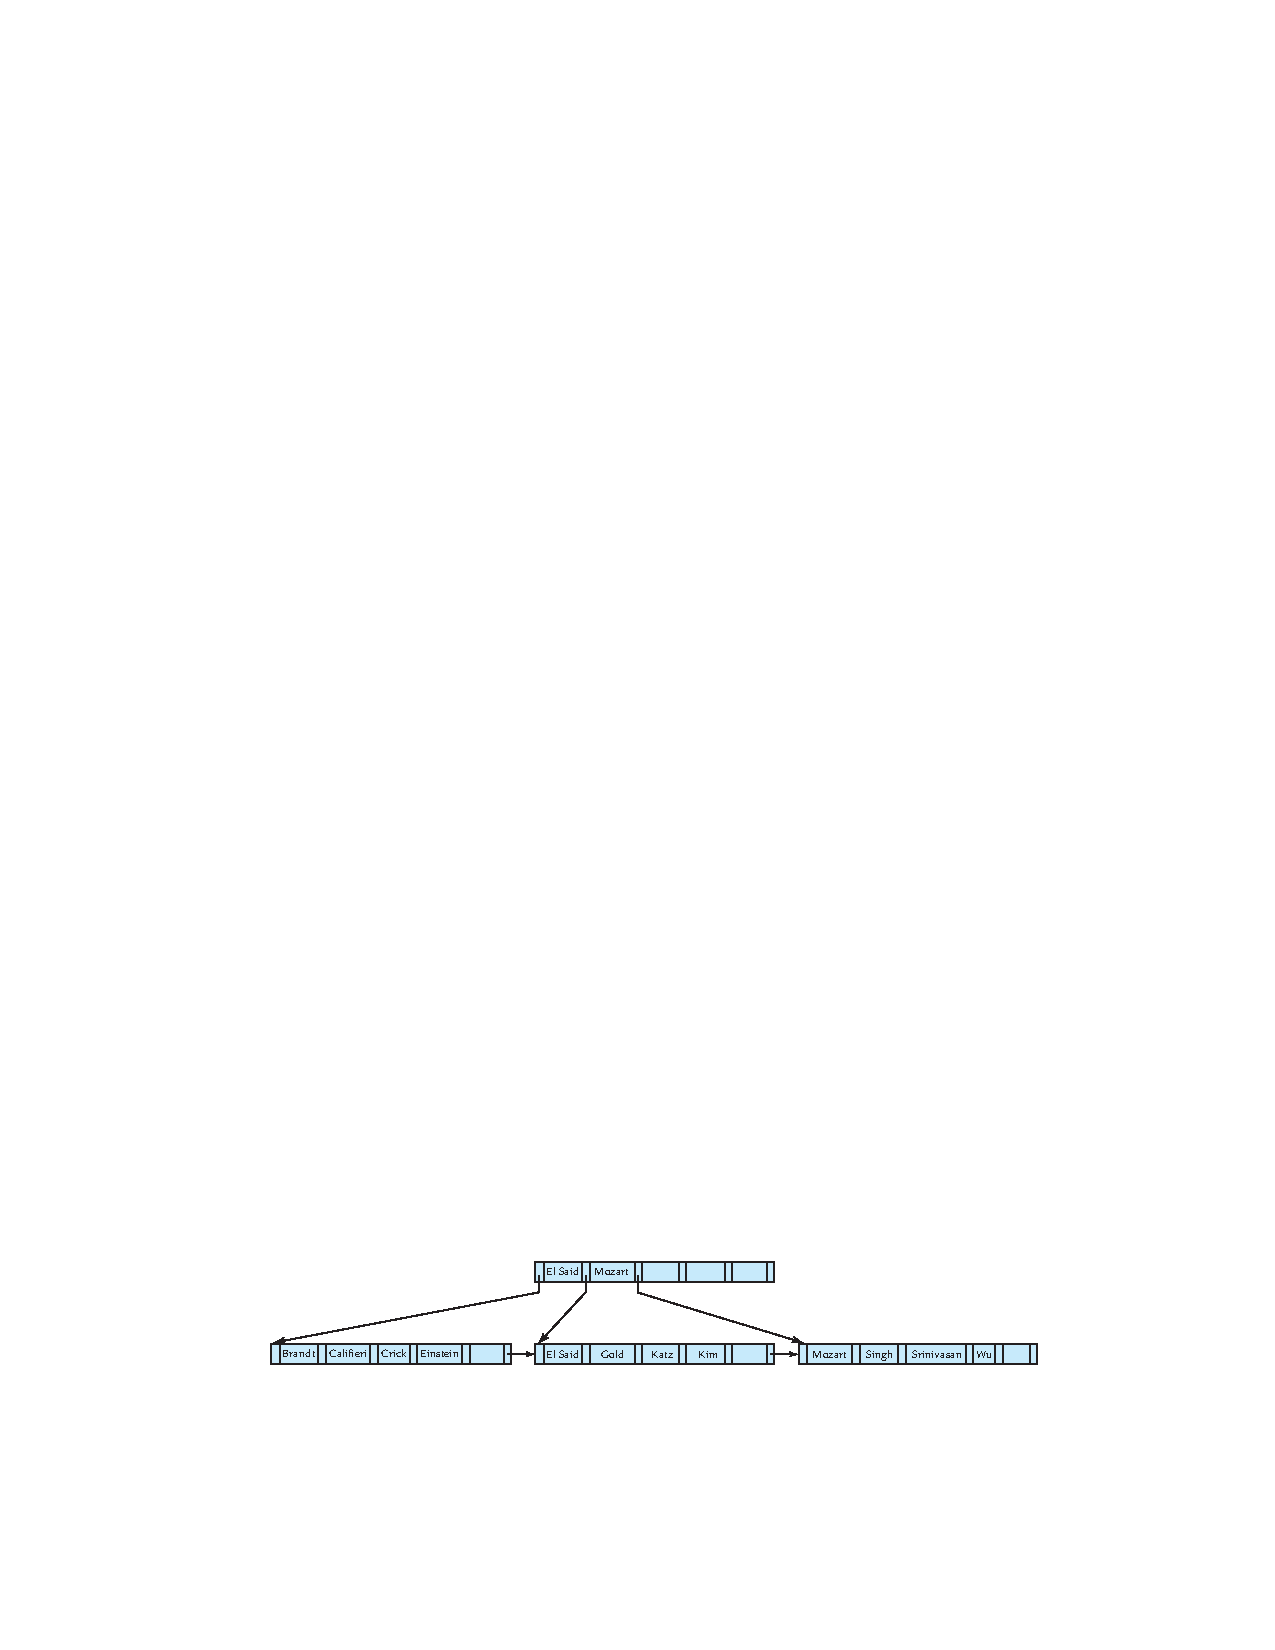
\includegraphics[width=0.8\textwidth]{aula06-btree4}
\caption{Árvore B+ com $n = 6$.}
\label{aula06:fig:btree4}
\end{figure}

Algums observações sobre árvores B+:
\begin{itemize}
\item Visto que as conexões entre nós são feitas por ponteiros, 
blocos ``logicamente'' próximos não precisam estar ``fisicamente'' 
próximos.

\item Os níveis não folha de uma árvore B+ formam uma hierarquia 
multinível de índices esparsos.

\item A árvore possui um número relativamente pequeno de níveis:
	\begin{itemize}
	\item O nível abaixo da raiz possui pelo menos $2 * \lceil n/2 \rceil$ valores.
	\item O próximo nível possui pelo menos $2 * \lceil n/2 \rceil * \lceil n/2 \rceil$ valores.
	\item ... etc.
	\item Se existem $K$ chaves de busca, a altura não é maior do que $\lceil \log_{n/2} K \rceil$.
	\item Por isso as buscas são eficientes.
	\end{itemize}
\item Inserções e remoções são eficientes, já que o índice é reestruturado em tempo 
logarítimico, como será visto adiante.
\end{itemize}

%%%%%%%%%%%%%%%%%%%%%%%%%%%%%%%%%%%%%%%%%%%%%%%%%%%%%%%%%%%%%%%%%%%%%%%%%%%%%%%
\subsection{Busca}

Os passos na busca em árvores B+ para uma chave de busca de valor $V$
onde retorna $C$ e o índice $i$ tal que $C.P_i$ aponta para o primeiro registro
com chave de busca $V$:
\begin{enumerate}
\item C = raiz.
\item \textbf{Repete} enquanto $C$ não é um nó folha:
	\begin{enumerate}
	\item Seja $i= $ o menor número tal que $V \leq C.K_i$.
	\item \textbf{Se} não existir um $i$, então $C = C.P_m$ onde $P_m$ é o último ponteiro não-nulo do nó.
	\item \textbf{Senão} (existe um $i$):
		\begin{enumerate}
		\item \textbf{Se} $V = C.K_i$, então $C = C.P_{i+1}$.
		\item \textbf{Senão} $C = C.P_i$ ($V < C.K_i$).
		\end{enumerate}
	\end{enumerate}
\item Seja $i$ o valor mínimo tal que $K_i = V$.
\item \textbf{Se} existe um $i$, retorna $(C, i)$, \textbf{senão} retorna $null$.
\end{enumerate}

Se o arquivo de índice possui $K$ chaves de busca, a altura da árvore não
ultrapassa $\lceil \log_{\lceil n/2 \rceil} K \rceil$
Um nó é geralmente do mesmo tamanho de um bloco, tipicamente $4$ Kbytes, e 
$n$ é tipicamente cerca de 100 (40 bytes por entrada no índice).
Com 1 milhão de chaves de busca e $n= 100$, no máximo $\log_{50}(1,000,000) = 4$
nós são acessados em uma busca, ou seja, no máximo 4 acessos a blocos.
Compare isso com uma árvore binária balanceada com 1 milhão de chaves de busca,
que acessa cerca de 20 nós em uma busca.
A diferença é significativa já que cada acesso a nó requer um acesso a disco.

%%%%%%%%%%%%%%%%%%%%%%%%%%%%%%%%%%%%%%%%%%%%%%%%%%%%%%%%%%%%%%%%%%%%%%%%%%%%%%%
\subsection{Atualização}

\subsubsection{Inserção}

Os passos para inserção em uma árvore B+ são:
\begin{enumerate}
\item Encontre o nó folha onde a chave de busca deveria aparecer.
\item Se a chave existir no nó folha:
	\begin{enumerate}
	\item Adicionar registro no arquivo.
	\item Adicionar o ponteiro no bucket.
	\end{enumerate}
\item Se a chave de busca não estiver presente:
	\begin{enumerate}
	\item Adicionar o registro no arquivo e criar o bucket.
	\item Se tiver espaço no nó folha, inserir par (chave, pointeiro).
	\item Senão, dividir o nó folha, junto com o novo par (chave-valor).
	\end{enumerate}
\end{enumerate}

A divisão do nó folha envolve os seguintes passos:
\begin{enumerate}
\item Pegar os $n$ pares (chave, apontador) (incluindo o novo) em ordem. Colocar os primeiros $\lceil n/2 \rceil$ no nó original e o restante no novo nó.
\item Considere que o novo nó é $p$, e $k$ é a menor chave em $p$. 
Inserir $(k,p)$ no pai do nó sendo dividido.
\item Se o pai estiver cheio, divida-o e propague a divisão para cima. A divisão prossegue até que se encontre um nó não cheio.
\end{enumerate}

No pior caso, a raiz será dividida, aumentando a altura da árvore em uma
unidade.

Os passos na divisão de um nó não folha, quando ao inserir $(k,p)$
em um nó interno $N$ já cheio, são:
\begin{enumerate}
\item Copiar $N$ para uma área temporária $M$ com espaço para $n+1$ pointeiros
e $n$ chaves.
\item Inserir $(k,p)$ em $M$.
\item Copiar $P_1,K_1, ..., K_{\lceil n/2 \rceil -1}, P_{\lceil n/2 \rceil}$ de
$M$ para o nó $N$. 
\item Copiar $P_{\lceil n/2 \rceil + 1}, K_{\lceil n/2 \rceil+1}, ..., K_n,
P_{n+1}$ de $M$ para o novo nó $N'$.
\item Inserir $(K_{\lceil n/2 \rceil},N')$ no pai $N$.
\end{enumerate}
A figura~\ref{aula06:fig:btree5} mostra um exemplo da divisão de um nó
não-folha cheio e inserção do no pai $N$.
%
\begin{figure}[!htb]
\centering
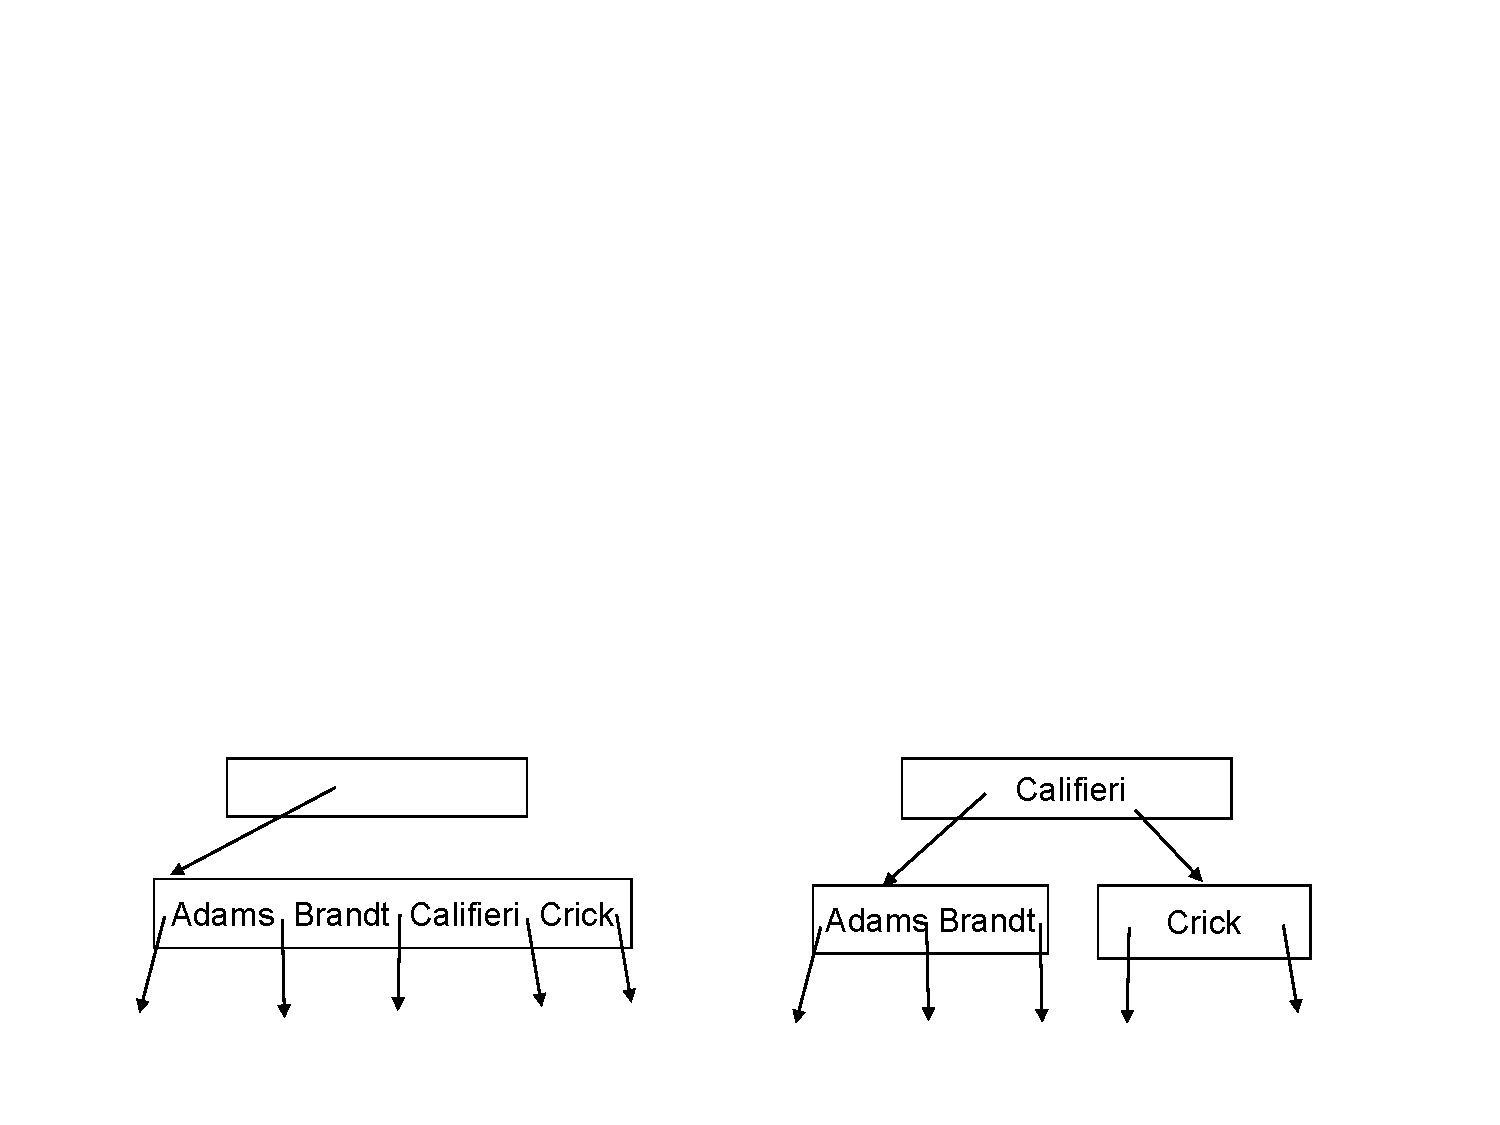
\includegraphics[width=0.7\textwidth]{aula06-btree5}
\caption{Exemplo de uma divisão de nó não-folha cheio.}
\label{aula06:fig:btree5}
\end{figure}

\subsubsection{Remoção}

%%%%%%%%%%%%%%%%%%%%%%%%%%%%%%%%%%%%%%%%%%%%%%%%%%%%%%%%%%%%%%%%%%%%%%%%%%%%%%%
\section{Índices Hash}
%%%%%%%%%%%%%%%%%%%%%%%%%%%%%%%%%%%%%%%%%%%%%%%%%%%%%%%%%%%%%%%%%%%%%%%%%%%%%%%

%%%%%%%%%%%%%%%%%%%%%%%%%%%%%%%%%%%%%%%%%%%%%%%%%%%%%%%%%%%%%%%%%%%%%%%%%%%%%%%
\section{Índices compostos}
%%%%%%%%%%%%%%%%%%%%%%%%%%%%%%%%%%%%%%%%%%%%%%%%%%%%%%%%%%%%%%%%%%%%%%%%%%%%%%%

%%%%%%%%%%%%%%%%%%%%%%%%%%%%%%%%%%%%%%%%%%%%%%%%%%%%%%%%%%%%%%%%%%%%%%%%%%%%%%%
\section{Índices de bitmap}
%%%%%%%%%%%%%%%%%%%%%%%%%%%%%%%%%%%%%%%%%%%%%%%%%%%%%%%%%%%%%%%%%%%%%%%%%%%%%%%

%%%%%%%%%%%%%%%%%%%%%%%%%%%%%%%%%%%%%%%%%%%%%%%%%%%%%%%%%%%%%%%%%%%%%%%%%%%%%%%
\section{Exercícios}
%%%%%%%%%%%%%%%%%%%%%%%%%%%%%%%%%%%%%%%%%%%%%%%%%%%%%%%%%%%%%%%%%%%%%%%%%%%%%%%

